%
%TODO: workout poisson noise
%
%TODO: workout conjugate gradients
%
%TODO: workout ransac
%
%TODO: workout belief propagation
\newcommand*{\E}{\bm{E}}
\newcommand*{\B}{\bm{B}}
\newcommand*{\rr}{\bm{r}}
\newcommand*{\Ef}{\textit{\textbf{E}} }
\section{Appendix}\label{sec:appendix}
\localtableofcontents

\subsection{Rayleigh Criterion}\label{subsec:rayleighcriterion}

We derive Rayleigh's criterion for the minimum angular resolution \(R_{min}\) of a \(\lambda\)-mono-chromatic point source through a \(D\)-diameter circular aperture
%
\begin{equation}
    R_{min} = 1.22 \frac{\lambda}{D} 
\end{equation}
%
from first principles.

\subsubsection{Wave Equation in a Vacuum}

Note this section primarily follows \cite{eom2004electromagnetic}.
%
Starting with Maxwell's equations in a vacuum (in differential form) for the electric field \(\E(x,y,z, t)\) and the magnetic field \(\B(x,y,z, t)\):
%
\begin{align}
    \nabla \times \B = \frac{1}{c^2} \frac{\partial \E}{\partial t} \\
    \nabla \times \E = - \frac{\partial \B}{\partial t}
\end{align}
%
Note that
%
\begin{equation}
    \nabla \times \left( \nabla \times \E \right) = \pd{}{t} \left( \nabla \times \B\right) = \frac{1}{c^2} \pdv[2]{\E}{t}
\end{equation}
%
and with the identity
\begin{equation}
    \nabla \times \nabla \times \E = \nabla (\nabla\cdot \E) - \nabla^2 \E
\end{equation}
%
we have the vector \(\bm{E}\)-field \newterm{vector wave equation}:
%
\begin{equation}
    \nabla^2 \E = \frac{1}{c^2} \pdv[2]{\E}{t}
\end{equation}
%
This decouples each components of the \(\bm{E}\) field. 
%
We therefore arbitrarily choose the \(z\) component \(E_z\) of \(\bm{E}\) and solve the \newterm{scalar wave equation} for \(E \coloneqq E_z\)
%
\begin{equation}
    \left(\nabla^2 - \frac{1}{c^2} \pdv[2]{}{t}\right) E = 0 \label{eqn:scalarwaveeqn}
\end{equation}
%

We proceed by \newterm{separation of variables}:
%
\begin{equation}
    E(\bx, t) = U(\bx) T(t)\label{eqn:sepvar}
\end{equation}
%
The solution for \(T\) is straightforward
%
\begin{equation}
    T(t) = e^{-\iu \omega t}
\end{equation}
%
where \(\omega = \beta c\) and \(\beta\) is separation constant.
%
\(U\) obeys the \newterm{Helmholtz equation}
%
\begin{equation}
    (\nabla ^{2}+\beta^{2})U=0\label{eqn:helmholtz}
\end{equation}
%
To solve for \(U\) we seek a \newterm{Green's function} \(G(\bx,\bx')\) of eqn.~\eqref{eqn:helmholtz}, i.e., \(G\) such that
%
\begin{equation}
    \nabla^2 G + \beta^2 G = -\delta(\bm{r})\label{eqn:helmgreen}
\end{equation}
%
where \(-\delta(\bm{r})\) is the \newterm{Dirac delta}\anote{diracdelta} centered at \(\bx'\) and \(\bm{r} = \bx - \bx'\).
%
Substituting the Fourier transform \(\tilde{G}(\bm{k})\) of \(G\)
%
\begin{equation}
    G(\bx, \bx') = \int\limits_{\mathbb{R}^3} \tilde{G} e^{\iu \bm{k}\cdot \bm{r}} \dif \bm{k}
\end{equation}
%
where \(\bm{k} = \left(k_1, k_2, k_3\right)\) and the Fourier representation of \(\delta(\bm{r})\)
\begin{equation}
    \delta(\bm{r}) = \int\limits_{\mathbb{R}^3} e^{\iu \bm{k} \cdot \bm{r}} \dif \bm{k}
\end{equation}
%
into eqn.~\eqref{eqn:helmgreen}
%
\begin{equation}
    \int\limits_{\mathbb{R}^3} \left(-k^2 +\beta^2 \right) \tilde{G}e^{\iu \bm{k}\cdot \bm{r}} \dif \bm{k} = - \int\limits_{\mathbb{R}^3} e^{\iu \bm{k}\cdot \bm{r}} \dif \bm{k}\label{eqn:helmgreenfourier}
\end{equation}
%
where \(k = \bm{k}\cdot\bm{k}\).
%
Comparing both sides of eqn.~\eqref{eqn:helmgreenfourier} we conclude that
%
\begin{equation}
    \tilde{G}(\bm{k}) = \frac{1}{k^2-\beta^2}
\end{equation}
%
and hence
%
\begin{equation}
    G(\bx, \bx') = \int\limits_{\mathbb{R}^3} \frac{e^{\iu \bm{k}\cdot \bm{r}}}{k^2-\beta^2}  \dif \bm{k}
\end{equation}
%
To compute this inverse Fourier transform, first rotate the \(\bm{k}\) coordinate system such that the \(k_3\)-axis and \(\bm{r}\) are aligned and then transform to spherical coordinates (see figure~\ref{fig:rotalign}).
%
\begin{figure}
    \tdplotsetmaincoords{60}{110}
    %
    \pgfmathsetmacro{\rvec}{.8}
    \pgfmathsetmacro{\thetavec}{30}
    \pgfmathsetmacro{\phivec}{60}
    %
    \begin{tikzpicture}[scale=5,tdplot_main_coords]
        \coordinate (O) at (0,0,0);
        \draw[thick,->] (0,0,0) -- (1,0,0) node[anchor=north east]{$k_1$};
        \draw[thick,->] (0,0,0) -- (0,1,0) node[anchor=north west]{$k_2$};
        \draw[thick,->] (0,0,0) -- (0,0,1) node[anchor=south]{$k_3$};

        \draw[thick,-stealth] (0,0,0) -- (0,0,.75) node[anchor=south west]{$\bm{r}$};
        \tdplotsetcoord{P}{\rvec}{\thetavec}{\phivec}
        \draw[-stealth,color=red] (O) -- (P) node[above right] {$\bm{k}$};
        \draw[dashed, color=red] (O) -- (Pxy);
        \draw[dashed, color=red] (0,0,.75) -- (P);
        \draw[dashed, color=red] (P) -- (Pxy);
        \tdplotdrawarc{(O)}{0.2}{0}{\phivec}{anchor=north}{$\phi$}
        \tdplotsetthetaplanecoords{\phivec}
        \tdplotdrawarc[tdplot_rotated_coords]{(0,0,0)}{0.5}{0}%
        {\thetavec}{anchor=south west}{$\theta$}
    \end{tikzpicture}
    \caption{Rotated/aligned spherical coordinate system for computing the inverse Fourier transform of \(\tilde{G}\).}\label{fig:rotalign}
\end{figure}
%
That implies
%
\begin{align*}
    \bm{k} \cdot \bm{r} & = k \abs{\bm{r}} \cos(\theta)
\end{align*}
%
and the differential volume element is
%
\begin{equation}
    \dif V = k^2 \sin(\theta) \dif \phi \dif \theta \dif k
\end{equation}
%
Then
%
\begin{multline}
    G(\bx, \bx') = \\
    \int\limits_{0}^\infty \int\limits_{0}^\pi  \int\limits_{0}^{2\pi}  \frac{e^{\iu k \abs{\bm{r}} \cos(\theta)}}{k^2-\beta^2} k \sin(\theta) \dif \phi \dif \theta \dif k = \\
    \frac{2\pi}{\iu \abs{\bm{r}}} \int\limits_{0}^{\infty}  \frac{e^{\iu k \abs{\bm{r}}} - e^{-\iu k \abs{\bm{r}}}}{(k - \beta)(k + \beta)} k \dif k \label{eqn:greensfn}
\end{multline}
%
Hence, since
%
\begin{equation}
    \int\limits_{0}^{\infty}  \frac{e^{\iu k \abs{\bm{r}}}}{(k - \beta)(k + \beta)} k \dif k
    =
    \int\limits_{-\infty}^{0}  \frac{ - e^{-\iu k \abs{\bm{r}}}}{(k - \beta)(k + \beta)} k \dif k
\end{equation}
%
equation~\eqref{eqn:greensfn} becomes
%
\begin{equation}
    G(\bx, \bx') =
    \frac{2\pi}{\iu \abs{\bm{r}}} \int\limits_{-\infty}^{\infty}  \frac{k e^{\iu k \abs{\bm{r}}}}{(k - \beta)(k + \beta)} \dif k \label{eqn:greenpole}
\end{equation}
%
Note that there are there are two singularities or \newterm{poles} in the integrand in eqn.~\eqref{eqn:greensfn}: the integrand goes to \(\infty\) as \(k\rightarrow +\beta\) or \(k\rightarrow -\beta\).
%
To perform the integral, despite the poles, we need to use complex integration and the residue theorem\anote{cauchyresidue}: we perform a line integral (called a \newterm{contour integral}) in the \(k\)-complex plane such that its value along the real axis equals the integral in eqn.~\eqref{eqn:greenpole} and its value elsewhere is zero.
%
\begin{figure}
    \centering
    \begin{tikzpicture}
        [
            decoration={%
                    markings,
                    mark=at position 0.5cm with {\arrow[line width=1pt]{>}},
                    mark=at position 2cm with {\arrow[line width=1pt]{>}},
                    mark=at position 0.5 with {\arrow[line width=1pt]{>}},
                    mark=at position 0.75 with {\arrow[line width=1pt]{>}},
                    mark=at position -5mm with {\arrow[line width=1pt]{>}},
                }
        ]
        \draw [help lines,->] (-4,0) -- (4,0) coordinate (xaxis);
        \draw [help lines,->] (0,-1) -- (0,4) coordinate (yaxis);
        \path [draw, line width=0.8pt, postaction=decorate]
        (-3,0) -- (3,0)
        node [anchor=north west] {} arc (0:180:3)
        node [anchor=north west] {};
        \node at (-2.6,-.4) {$C_1$};

        \node [below] at (xaxis) {$\operatorname{Re}\{k\}$};
        \node [left] at (yaxis) {$\operatorname{Im} \{k\}$};


        \node [font=\scriptsize, anchor=north] at (1.5,0) {$+\beta$};
        \node [] at (1.5,0) {$\times$};
        \node at (1.5,.7) {$\times$};
        \draw [dashed] (1.5,0) -- (1.5,.7);
        \node [font=\scriptsize] at (1.5,1) {$+\beta+\iu\epsilon$};

        \node [font=\scriptsize, anchor=south] at (-1.5,0) {$-\beta$};
        \node [] at (-1.5,0) {$\times$};
        \node at (-1.5,-.7) {$\times$};
        \draw [dashed] (-1.5,0) -- (-1.5,-.7);
        \node [font=\scriptsize] at (-1.5,-1) {$-\beta-\iu\epsilon$};

        \node at (3,1.8) {$C_2$};
        \draw [-stealth] (0,0) -- (1,2.85) node[midway, left] {$R$};
    \end{tikzpicture}
    \caption{Contour \(C = C_1 \cup C_2\) for the Helmholtz Green's function contour integral with poles \(-\beta, +\beta\) and shifted poles \(-\beta -\iu \epsilon, +\beta + \iu \epsilon\).}\label{fig:helmcontour}
\end{figure}

A critical requirement of the residue theorem is that the poles are wholly contained in the contour.
%
To that end we shift the poles \(-\beta,+\beta\) by a pure imaginary component \(+\iu \epsilon\) and then ultimately take the limit of the result of the perturbed integral as \(\epsilon \rightarrow 0\).
%
Consider the contour \(C\) in figure~\ref{fig:helmcontour}.
%
It's composed of the portion \(C_1\) along \(\operatorname{Re} \{k\}\) and the semi-circle \(C_2\) in the positive \(\operatorname{Im} \{k\}\) half-plane.
%
If we take the limit as \(R \rightarrow \infty\) then the integral along \(C_1\) agrees with the integrand in eqn.~\eqref{eqn:greenpole} and by \newterm{Jordan's lemma}\anote{jordanlemma}, with 
%
\[
    g(k)=\frac{1}{k^2 - \beta^2}
\]
%
the integral along \(C_2\) vanishes.
%
Therefore
%
\begin{align}
    G(\bx, \bx') & = \lim_{\epsilon \rightarrow 0}  \frac{(2\pi)^2}{\abs{\bm{r}}} \operatorname {Res} (f, \beta+\iu \epsilon)                       \\
                 & = \frac{(2\pi)^2}{\abs{\bm{r}}} \lim_{\epsilon \rightarrow 0} \frac{\beta e^{\iu \beta \abs{\bm{r}}}}{ 2(\beta + \iu \epsilon) } \\
                 & = A \frac{e^{\iu \beta \abs{\bm{r}}}}{\abs{\bm{r}} } \\ 
                 & = A \frac{e^{\iu k r}}{r} \label{eqn:helmholtzsoln}
\end{align}
%
where \(A\) absorbs constant factors, \(r = \abs{\bm{r}}\), and \(k \equiv \beta\) to better align with conventional notation.
%
% \begin{equation}
%     \frac{e^{\iu k \abs{\bx -\bx'}}}{4 \pi \abs{\bx - \bx'}}\label{eqn:helmholtzsoln}
% \end{equation}
% %
%
Finally, recalling eqn.~\eqref{eqn:sepvar}, we have the \newterm{mono-chromatic spherical wave} solution\footnote{So named due to the spherical symmetry of the solution, i.e., dependence on only \(r\) and a single frequency \(\omega\)}:
%
\begin{equation}
    E(r, t) = A\frac{e^{\iu (k r - \omega t)}}{r}\label{eqn:sphericalwavesoln}
\end{equation}
%

\subsubsection{Kirchhoff-Helmholtz integral theorem}

\begin{figure*}
    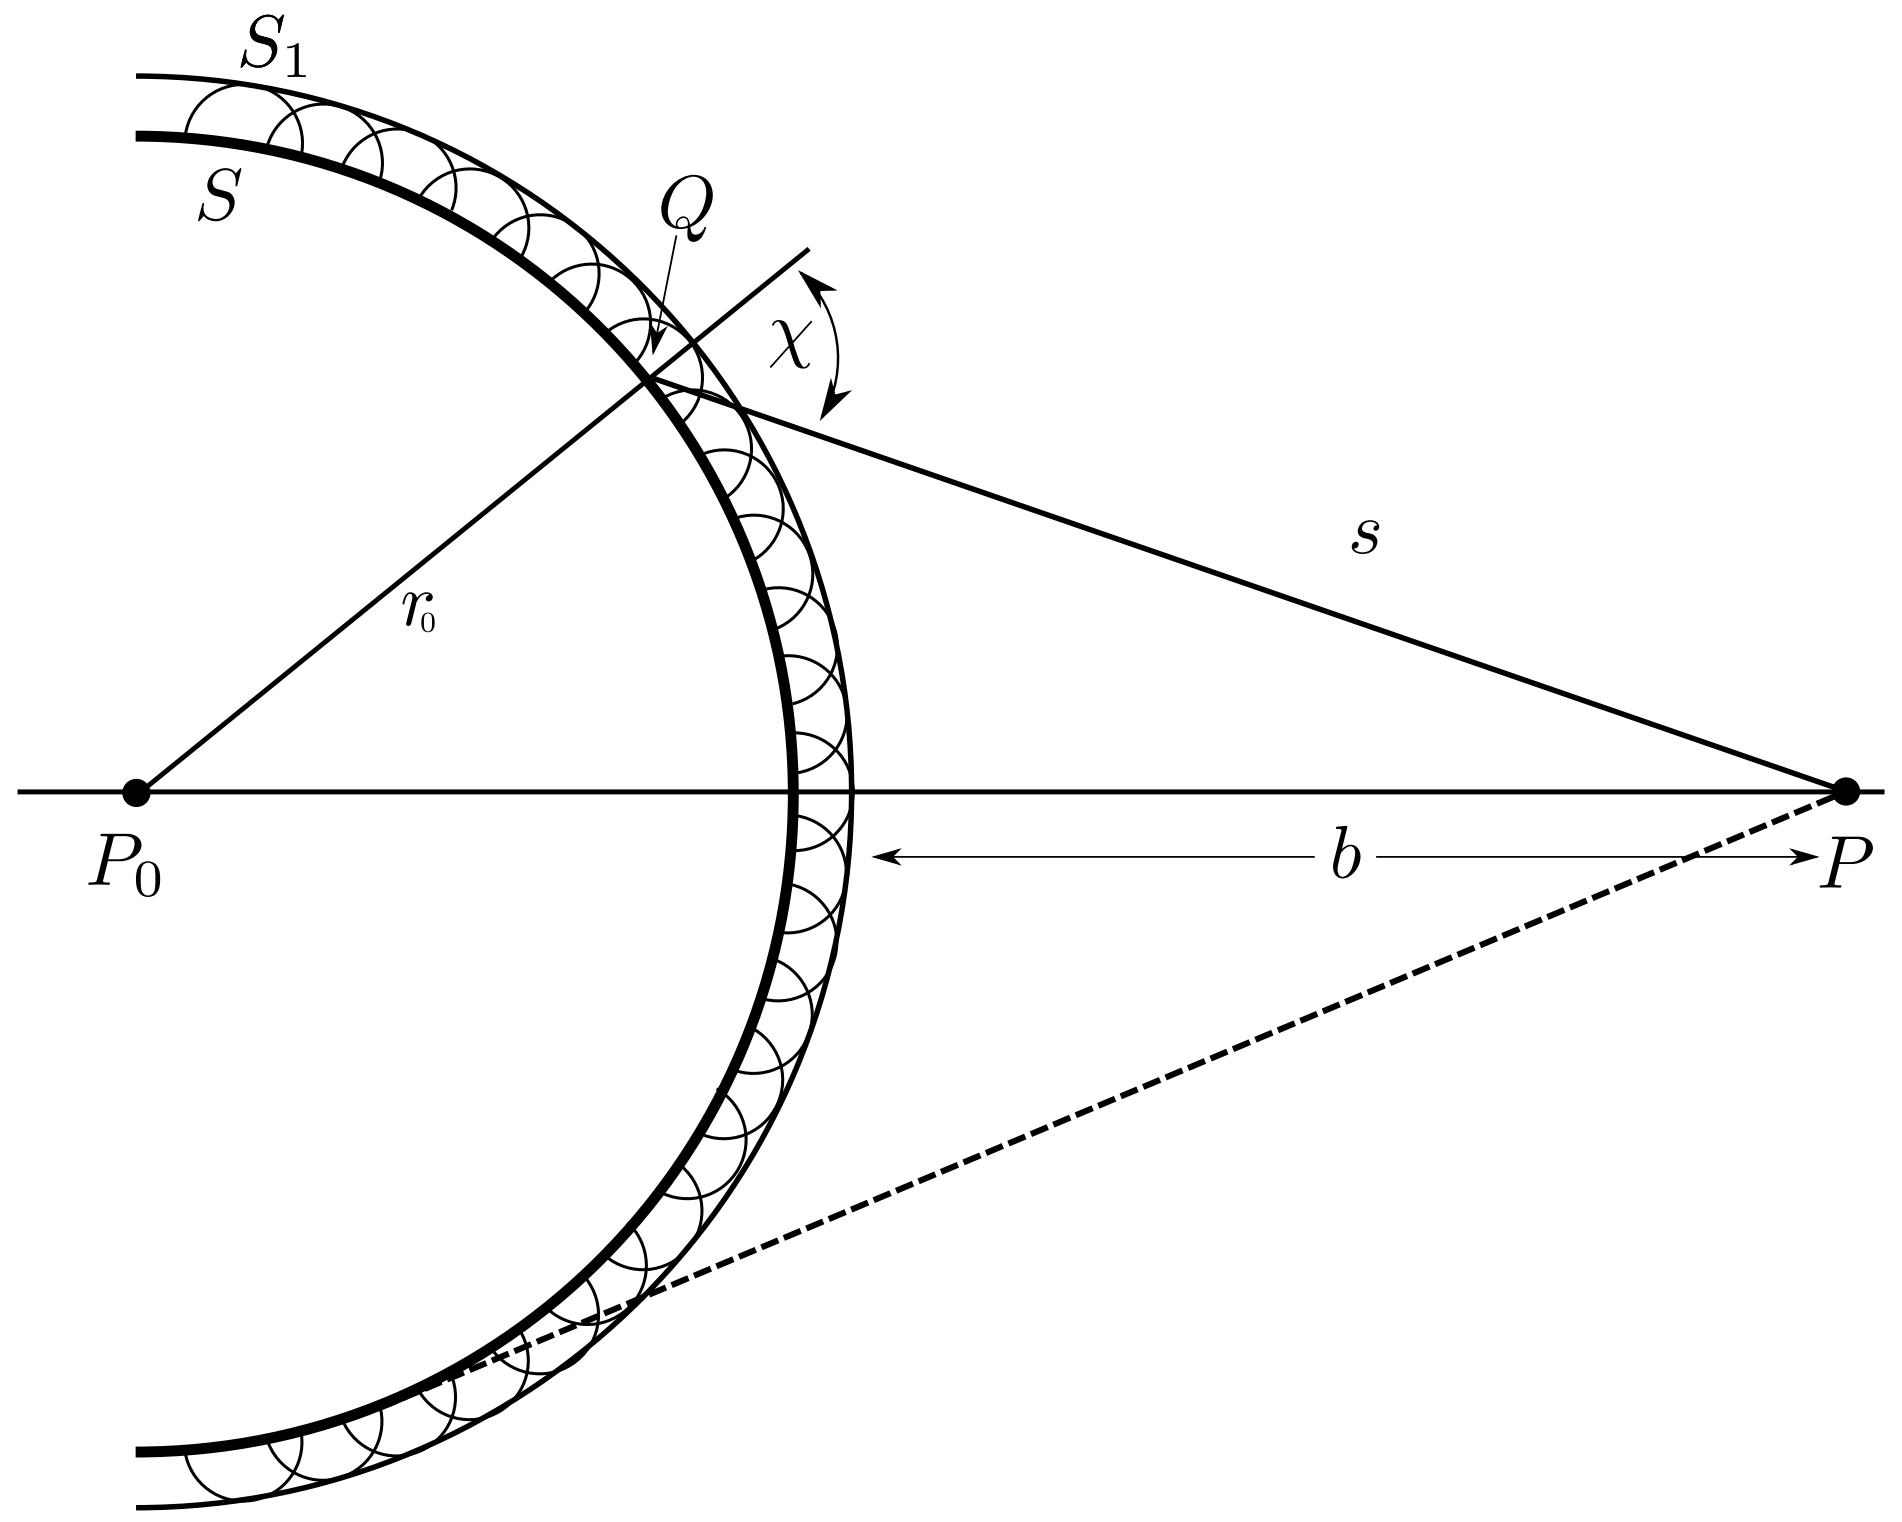
\includegraphics[width=\textwidth]{figures/appendix/huygens-fresnel.png}
    \caption{Illustration of the Huygens-Fresnel principle. \(P_0\) and \(P\) are the light source and the receiver, respectively, \(r_0\) is the
        radius of the wave front with surface \(S,S_1\) is the wave front at a later instant and \(\chi\) is the inclination angle at some point
        \(Q\) \cite{Ivanov2016ElementsOD}.}\label{fig:huygensfresnel}
\end{figure*}
Note this section and the proceeding ones closely follows \cite{Ivanov2016ElementsOD}.
%
Let \(P_0\) be a point source emitting spherical waves and \(S\) an arbitrary spherical wave-front with radius \(r_0\).
%
According to the \newterm{Huygens-Fresnel principle} each point \(Q\) on \(S\) is a secondary emitter.
%
Consider figure~\ref{fig:huygensfresnel} and let \(S_1\) be the secondary wave-front (envelope of secondary emitters).
%
Then the field at a distant point \(P\) is the superposition of secondary waves that originate from the surface \(S\).
%
Kirchoff's derived Huygens-Fresnel by computing the field at point \(P\) in terms of only the field
and its derivatives at points on an arbitrary surface enclosing \(P\) (see figure~\ref{fig:kirchoff}) using an \textit{auxiliary function} \(U'\).
%
\begin{figure}
    \centering 
    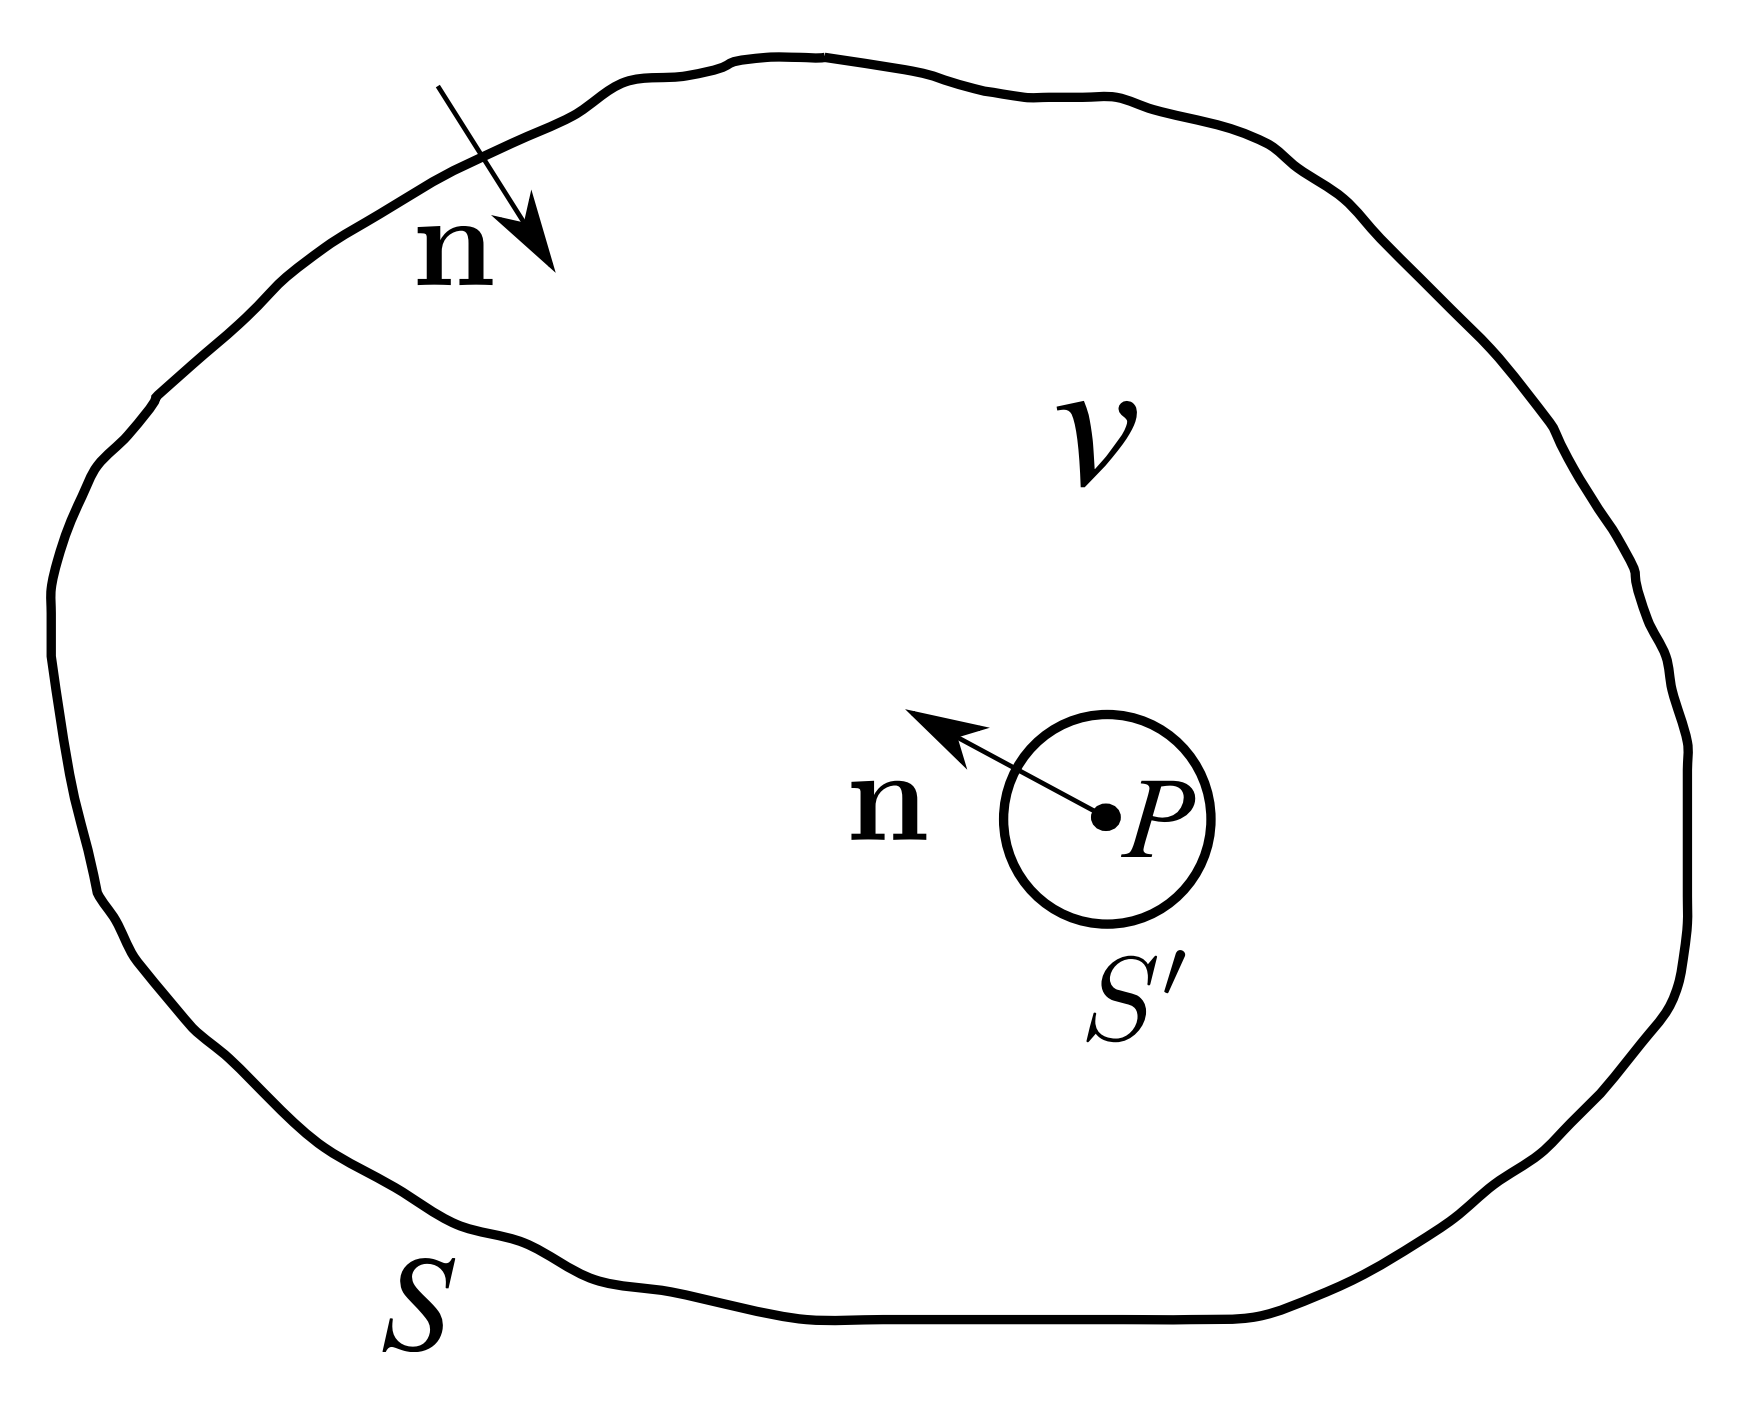
\includegraphics[width=\linewidth]{figures/appendix/kirchoff.png}
    \caption{Schematic for derivation of Kirchhoff-Helmholtz integral \cite{Ivanov2016ElementsOD}.}\label{fig:kirchoff}
\end{figure}

First we derive a general fact about fields; if we assume two fields \(U, U'\) are continuously differentiable to second order on \(S\) (and on its interior) then we have by \newterm{Green's theorem}\anote{greenstheorem}
%
\begin{multline}
    \int\limits_{v}\left(U \nabla^2 U' - U' \nabla^2 U \right)\,dV = \\ - \int\limits_{S}\left(U \pdv{U'}{\bm{n}}- U'  \pdv{U}{\bm{n}}\right)\,\dif S\label{eqn:greensequal}
\end{multline}
%
where \(\pdv{}{\bm{n}}\) is the directional derivative in the direction of the \textbf{inward}\footnote{We use inward rather than outward in order to handle a forthcoming nuance.} pointing normal \(\bm{n}\).
%
Then, since \(U, U'\) both satisfy eqn.~\eqref{eqn:helmholtz}, the left-hand side of eqn.~\eqref{eqn:greensequal} vanishes and we have that
%
\begin{equation}
    \int\limits_{S}\left(U \pdv{U'}{\bm{n}} - U'  \pdv{U}{\bm{n}}\right)\,\dif S = 0
    \label{eqn:greenssimple}
\end{equation}

Suppose now that the auxiliary function \(U'\) is the Helmholtz Green's function (eqn.~\eqref{eqn:helmholtzsoln})
%
\begin{equation}
    U' = \frac{e^{\iu k s}}{s}
\end{equation}
%
That is to say, to be the field at a secondary emitter on the wave-front\footnote{\(s\) being the distance from \(P\) to the emitter as in figure~\ref{fig:huygensfresnel}}.
%
Note that \(U'\) has a singularity at \(s = 0\) (i.e. at \(P\)); since an assumption of eqn.~\eqref{eqn:greensequal} is that \(U'\) is continuous and differentiable in the entire volume \(v\), we must exclude \(P\) from the domain of integration.
%
We shall therefore surround \(P\) by a small sphere \(S'\) of radius \(\epsilon\), treat the integration on the left-hand side eqn.~\eqref{eqn:greensequal} as \textbf{over the volume between the exterior surface \(S\) and the interior surface \(S'\)}, and then take the limit as \(\epsilon \rightarrow 0\).

Hence the integration in eqn.~\eqref{eqn:greenssimple}
%
\begin{equation}
    \left\{ \int\limits_{S} + \int\limits_{S'} \right\} \left[U \pdv{}{\bm{n}} \frac{e^{\iu k s}}{s} - \frac{e^{\iu k s}}{s} \pdv{U}{\bm{n}}\right]\,\dif S = 0
\end{equation}
%
Note that surface normal \(\bm{n}\) points inwardly (into the volume) at both surfaces.
%
Therefore
%
\begin{multline}
    \int\limits_{S} U \pdv{}{\bm{n}} \frac{e^{\iu k s}}{s} - \frac{e^{\iu k s}}{s} \pdv{U}{\bm{n}} \dif S = \\
    - \int\limits_{S'} \left( U \frac{e^{\iu k s}}{s} \left( \iu k  - \frac{1}{s} \right) - \frac{e^{\iu k s}}{s} \pdv{U}{\bm{n}} \right) \dif S = \\
    - \int\limits_{\Omega} \left( U \frac{e^{\iu k \epsilon}}{\epsilon} \left( \iu k  - \frac{1}{\epsilon} \right) - \frac{e^{\iu k \epsilon}}{\epsilon} \pdv{U}{\bm{n}} \right)\epsilon^2 \dif \Omega \label{eqn:solidangle}
\end{multline}
%
where \(\dif \Omega\) is differential \newterm{solid angle}\anote{solidangle} and we have used the fact
%
\begin{multline}
    \pdv{}{\bm{n}} \frac{e^{\iu k s}}{s} = \bm{n}\cdot \nabla \left( \frac{e^{\iu k s}}{s} \right) = \\ \bm{n} \cdot \hat{\bm{s}} \left( \pdv{}{s} \frac{e^{\iu k s}}{s}\right) =  \pdv{}{s} \frac{e^{\iu k s}}{s}
\end{multline}
%
since \(\bm{n} \cdot \hat{\bm{s}} = 1\) (since \(S'\) is a sphere).
%
Taking the limit of the right-hand side of eqn.~\eqref{eqn:solidangle} we see that terms proportional to \(\epsilon\) don't contribute (first and third) and therefore
%
\begin{align}
    \int\limits_{S} \left( U \pdv{}{\bm{n}} \frac{e^{\iu k s}}{s} - \frac{e^{\iu k s}}{s} \pdv{U}{\bm{n}} \right) \dif S & = \lim_{\epsilon \rightarrow 0} \int\limits_{\Omega} U e^{\iu k \epsilon} \dif \Omega \\
                                                                                                          & = 4 \pi U(P)
\end{align}
%
since \(\lim_{\epsilon \rightarrow 0} e^{\iu k \epsilon} = 1\) and the integration over \(\dif \Omega\) doesn't depend on \(\epsilon\).
%
Therefore the field \(U\) at point \(P\) is determined by the \newterm{Kirchhoff-Helmholtz integral theorem}
%
\begin{equation}
    U(P) = \frac{1}{4 \pi}\int\limits_{S} \left( U \pdv{}{\bm{n}} \frac{e^{\iu k s}}{s} - \frac{e^{\iu k s}}{s} \pdv{U}{\bm{n}} \right) \dif S \label{eqn:kirchoffhelmintegral}
\end{equation}
%
Note that the Kirchhoff-Helmholtz integral theorem determines \(U(P)\) as a function of the values of \(U\) and \(\partial U / \partial \bm{n}\) on the surface \(S\) alone.

\subsubsection{Fresnel-Kirchhoff diffraction}

\begin{figure}
    \centering
    \newcommand*{\subfigwidth}{\linewidth}
    \begin{subfigure}[b]{\subfigwidth}
        \centering
        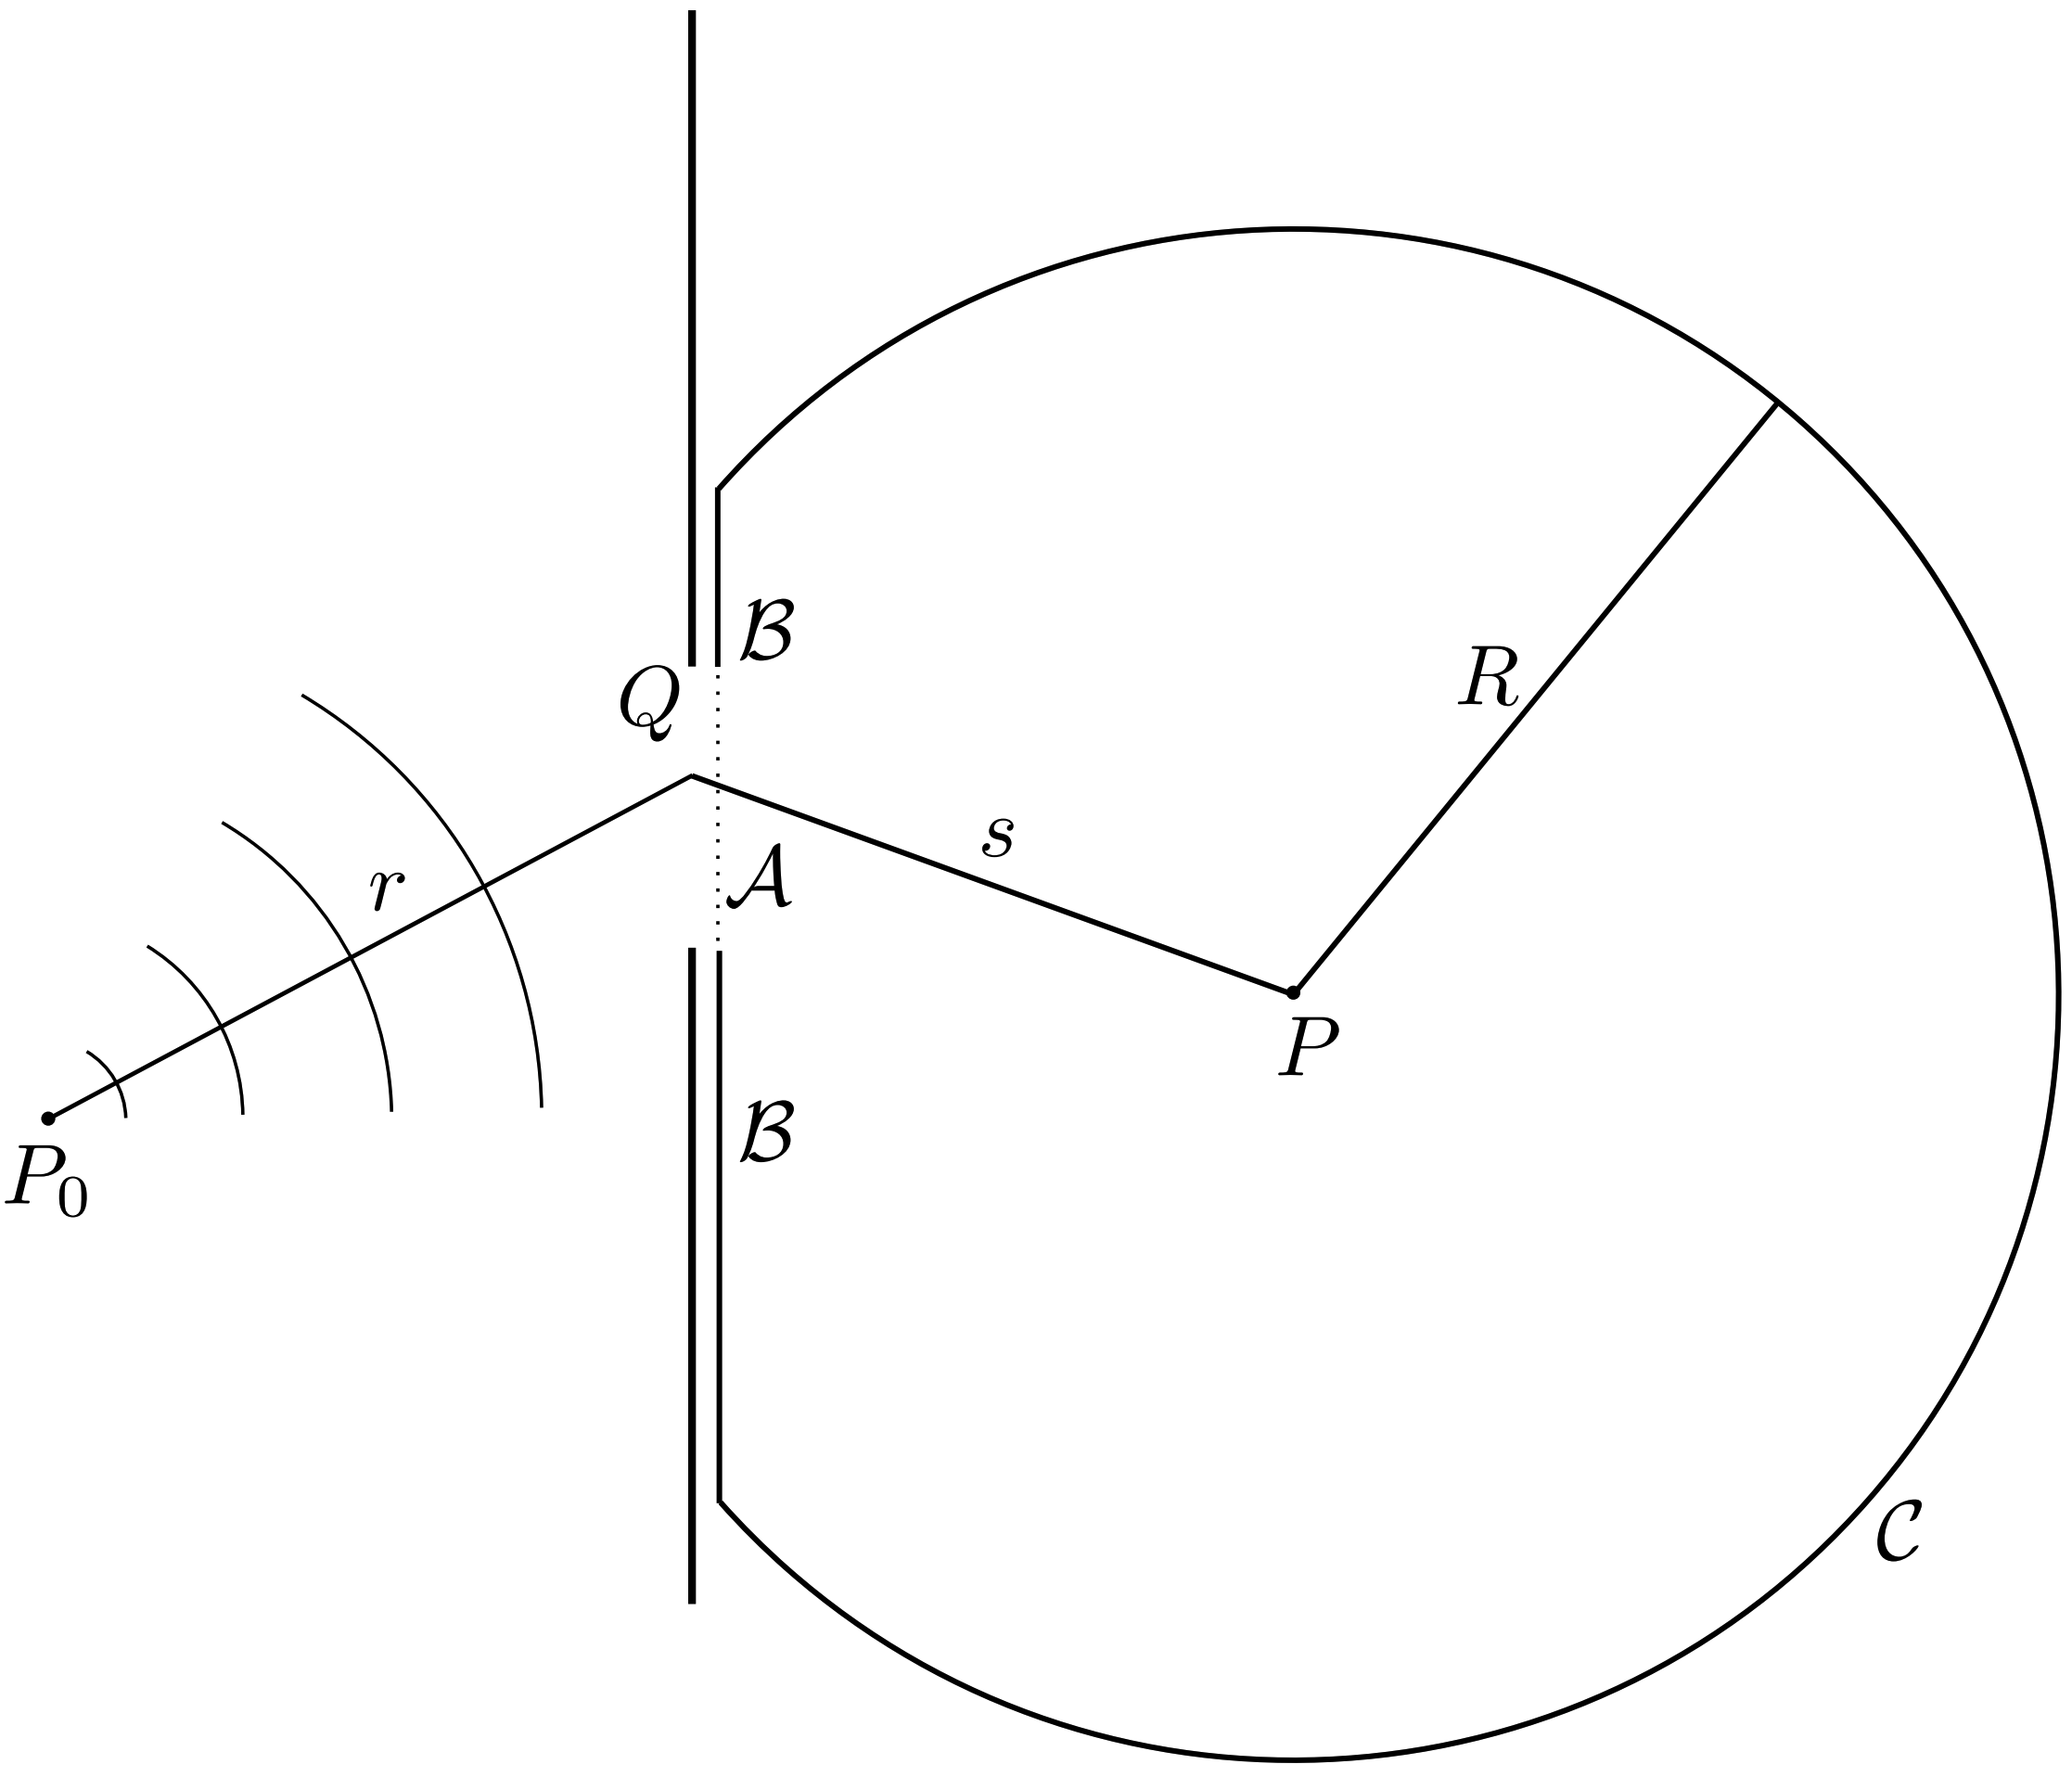
\includegraphics[width=\linewidth]{figures/appendix/fresnel-kirchoff.png}
        \caption{The surface \(S\) consists of portions \(\mathcal{A}, \mathcal{B}, \mathcal{C}\) \cite{Ivanov2016ElementsOD}.}\label{subfig:fresnelkirchoffsurf}
    \end{subfigure}
    \vskip\baselineskip
    \begin{subfigure}[b]{\subfigwidth}
        \centering
        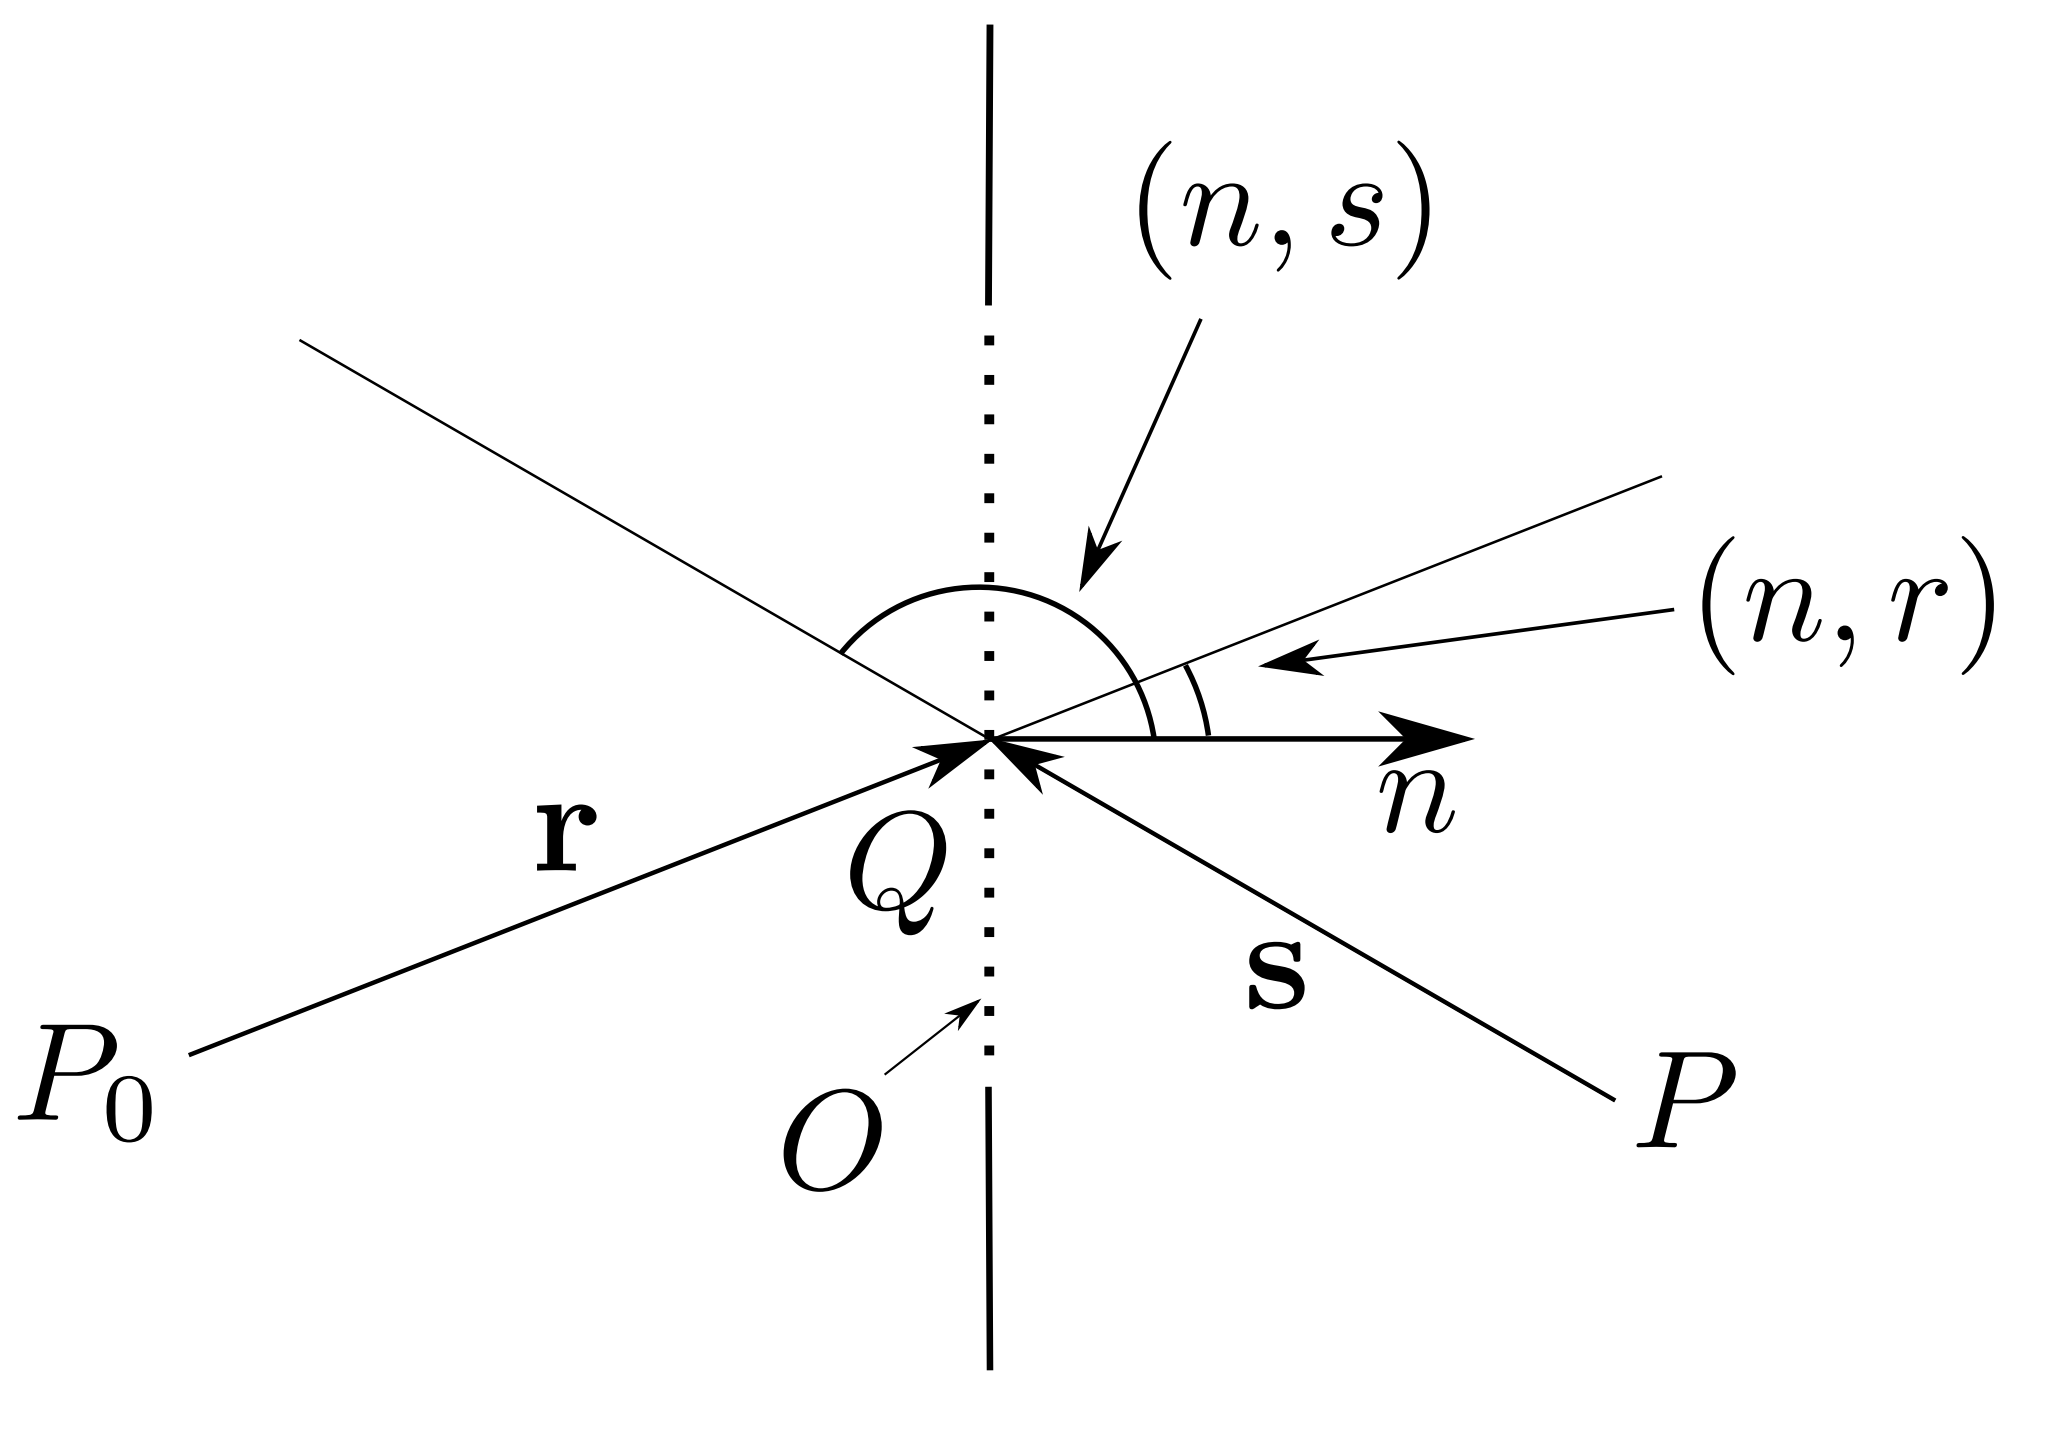
\includegraphics[width=\linewidth]{figures/appendix/fresnelkirchoffsetup.png}
        \caption{Definition of angles and directions. \textbf{r} and \textbf{s} point in the direction of increasing \textit{r}
        and \textit{s}, respectively, and \textbf{n} is normal to the screen. \((n,s)\) and \((n,r)\) indicate the angles between the normal \(\bm{n}\) and \(\bm{s}, \bm{r}\) respectively \cite{Ivanov2016ElementsOD}.}\label{subfig:fresnelkirchoffangles}
    \end{subfigure}
    \caption{Illustrating the derivation of the Fresnel-Kirchhoff diffraction formula of propagation through an aperture.}\label{fig:fresnelkirchoff}
\end{figure}

We now apply eqn.~\eqref{eqn:kirchoffhelmintegral} to the typical case of waves propagating through an aperture in a screen (see figure~\ref{subfig:fresnelkirchoffsurf}).
%
We take as our surface \(S = \mathcal{A} \cup \mathcal{B} \cup \mathcal{C}\) where \(\mathcal{A}\) is the aperture itself, \(\mathcal{B}\) is the unilluminated side of the screen, and \(\mathcal{C}\) is a portion of a large sphere centered at \(P\).
%
The Kirchhoff-Helmholtz integral dictates that 
%
\begin{equation}
    U(P) = \frac{1}{4 \pi} \left\{ \int\limits_{\mathcal{A}}  + \int\limits_{\mathcal{B}} + \int\limits_{\mathcal{C}}  \right\} \left[ U \pdv{}{\bm{n}} \frac{e^{\iu k s}}{s} - \frac{e^{\iu k s}}{s} \pdv{U}{\bm{n}} \right] \dif S
\end{equation}
%
Note that a fortiori the field is \(\sim\,\)0 on \(\mathcal{B}\) because it is unilluminated.
%
Similarly we'd hope the field on \(\mathcal{C}\) is approximately zero as well, since we are free to choose \(R\) as large as we want.
%
Unfortunately, this isn't exactly the case; while it is true that both \(U, \partial U/ \partial \bm{n} \rightarrow 0\) as \(R \rightarrow \infty\) it's also the case that the area of \(S \rightarrow \infty\) and so we don't necessarily have that the integral on \(\mathcal{C}\) vanishes.
%
To assure this we need to further assume \newterm{Sommerfeld’s radiation condition}:
%
\begin{equation}
    \lim_{R \rightarrow \infty} R \left( U(R) - \pdv{U}{\bm{n}} \right)  = 0
\end{equation}
%
which assumes we are only dealing with \textit{outgoing} waves.
%
With this assumption included the integral on \(\mathcal{C}\) indeed vanishes.

This leaves the field on \(\mathcal{A}\).
%
Kirchoff assumed that the field on \(\mathcal{A}\) is the same as if the screen were absent, i.e., the field is determined by a spherical wave emanating from \(P_0\) (see eqn.~\eqref{eqn:helmholtzsoln}).
%
Therefore we have 
%
\begin{align}
    U(P) &= \frac{1}{4 \pi}\int\limits_{S} \left( U \pdv{}{\bm{n}} \frac{e^{\iu k s}}{s} - \frac{e^{\iu k s}}{s} \pdv{U}{\bm{n}} \right) \dif S  \\ 
    &= \frac{A}{4 \pi}\int\limits_{\mathcal{A}} \left( \frac{e^{\iu k r}}{r} \pdv{}{\bm{n}} \frac{e^{\iu k s}}{s} - \frac{e^{\iu k s}}{s} \left(\pdv{}{\bm{n}} \frac{e^{\iu k r}}{r}\right) \right) \dif S
\end{align}
%
Assuming the wavelength of the field is much smaller than the distances involved (\(\lambda \ll r, s\) both and therefore \(k \gg 1/r, 1/s\) both), we can approximate 
\[
  \iu k - \frac{1}{r} \approx \iu k - \frac{1}{s} \approx \iu k  
\]
%
Then the \newterm{Fresnel-Kirchhoff diffraction formula} reads
\begin{align}
    U(P) &= \frac{1}{4 \pi}\int\limits_{S} \left( U \pdv{}{\bm{n}} \frac{e^{\iu k s}}{s} - \frac{e^{\iu k s}}{s} \pdv{U}{\bm{n}} \right) \dif S  \\ 
    &= \frac{\iu A}{2 \lambda}\int\limits_{\mathcal{A}}  \left( \frac{e^{\iu k (r+s)}}{r s} \left(\cos(n, s) - \cos(n, r) \right) \right) \dif S \label{eqn:fresnelkirchoff}
\end{align}
%
where \((n, s)\) is the angle between \(\bm{n}\) and \(\bm{s}\) and similarly \((n, r)\) (see figure~\ref{subfig:fresnelkirchoffangles}).

\subsubsection{Fraunhofer Diffraction}

\begin{figure}
    \centering 
    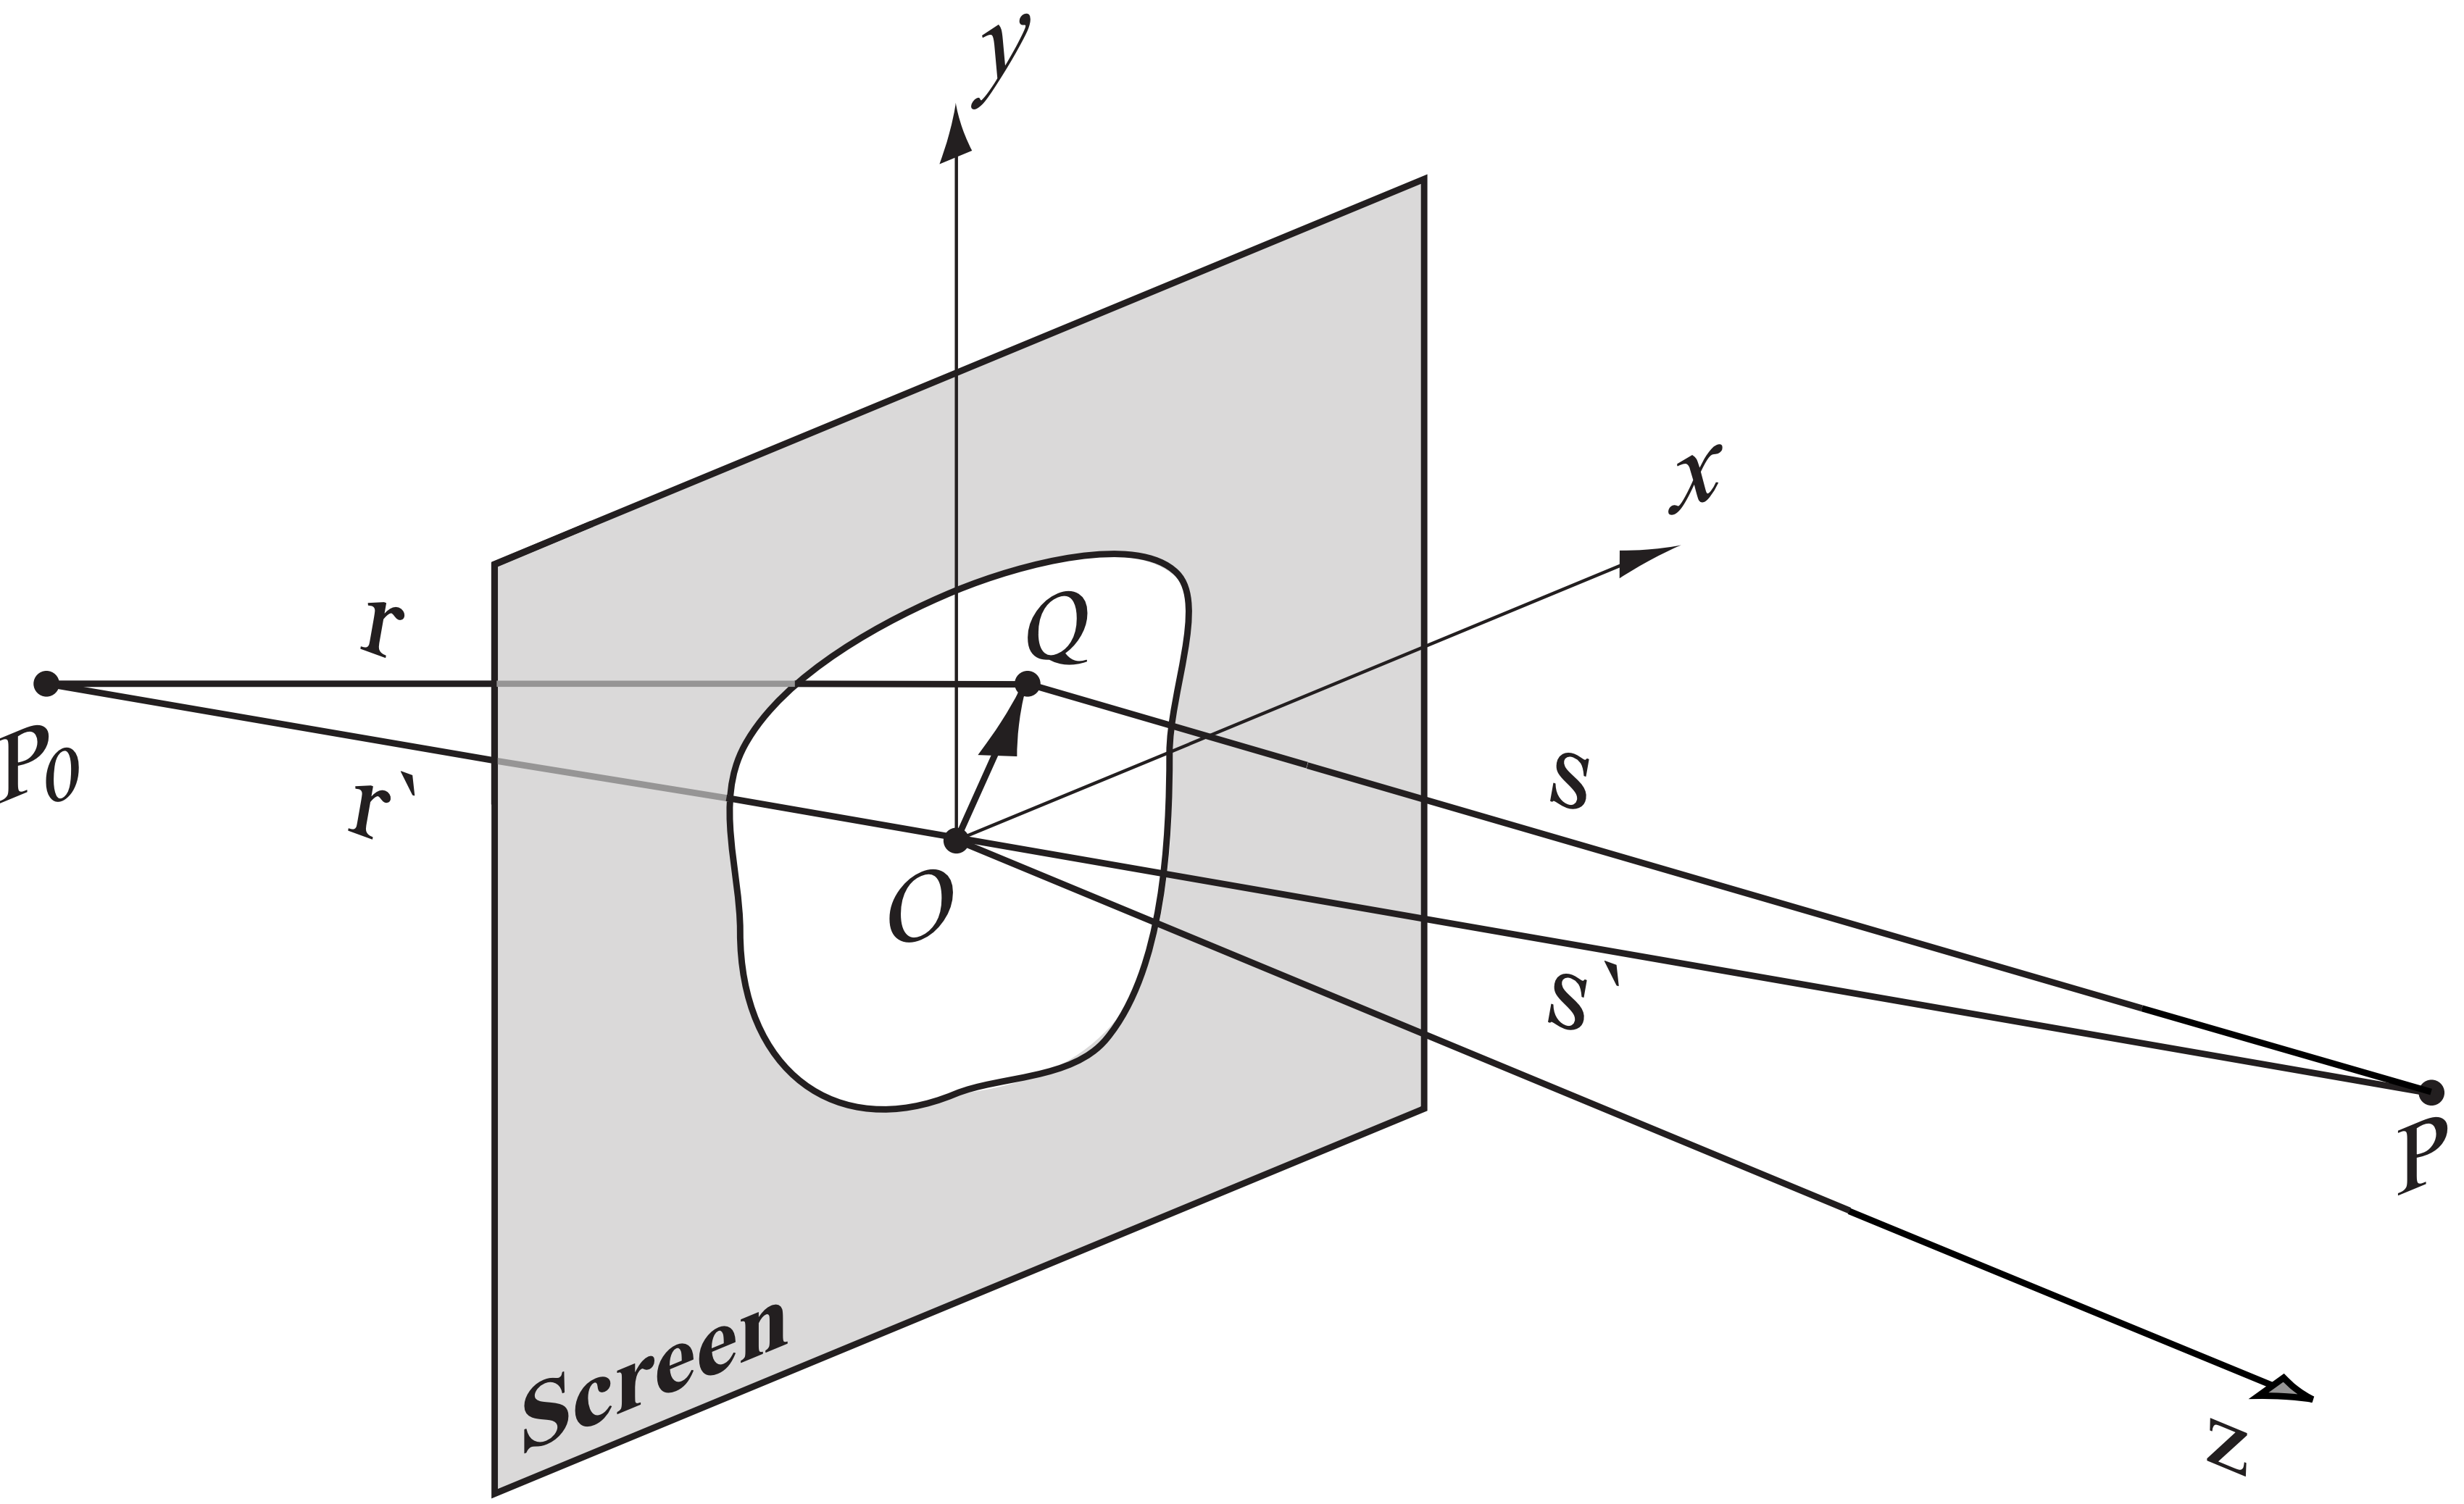
\includegraphics[width=\linewidth]{figures/appendix/plane-screen.png}
    \caption{Diffraction at an aperture in a plane screen. We introduce Cartesian coordinates with origin \(O\), where the \(xy\)-plane
    and the aperture plane coincide and positive \(z\) direction points into the half-space containing \(P\). An arbitrary point \(Q\) within
    the aperture is specified by the coordinates \(\xi, \eta\) \cite{Ivanov2016ElementsOD}.}\label{fig:planescreen}
\end{figure}

We now make further assumptions in order to be able to evaluate eqn.~\eqref{eqn:fresnelkirchoff} analytically.
%
Assume that the dimensions of the opening are large compared to \(\lambda \) but are small compared to \(r,s\). 
%
That is to say, \(\lambda \ll a \ll r,s\) where \(a\) is the characteristic size of the aperture (radius or edge length).

%
The assumption \(a \ll r,s\) implies \(\cos(n, s) - \cos(n, r)\) varies very little over the aperture (see figure~\ref{fig:planescreen}) and hence
\begin{equation}
    \cos(n, s) - \cos(n, r) \approx  \cos(n, s') - \cos(n, r')
\end{equation}
%
and similarly \(1/rs \approx 1/r's'\).
%
Hence
%
\begin{equation}
    U(P) \approx \frac{\iu A}{2 \lambda} \frac{\left(\cos(n, s') - \cos(n, r') \right) }{r's'}\int\limits_{\mathcal{A}} e^{\iu k (r+s)} \dif S \label{eqn:fresnelapprox}
\end{equation}

The integral in eqn.~\eqref{eqn:fresnelapprox} is still only numerically computable and so we make further assumptions in order to approximate \(e^{\iu k (r+s)}\).
%
First, we introduce a Cartesian coordinate system with origin \(O\) in the aperture, with the \(xy\)-axes in the plane of the aperture.
%
We then choose the positive \(z\) direction to point into the half-space that contains the point \(P\) (see figure~\ref{fig:planescreen}).
%
Let \(P_0 = (x_0, y_0, z_0)\), \(P = (x,y,z)\), and an arbitrary point \(Q = (\xi, \eta)\) in the aperture plane.
%
Then
%
\begin{align}
    r^2 &= (x_0-\xi)^2 + (y_0 - \eta)^2 + z_0^2 \\
    s^2 &= (x-\xi)^2 + (y - \eta)^2 + z^2 \\
    (r')^2 &= x_0^2 + y_0^2 + z_0^2 \\
    (s')^2 &= x^2 +y^2 + z^2 
\end{align}
%
and hence
%
\begin{align}
    r^2 &=  (r')^2 - 2 (x_0 \xi + y_0 \eta) + \xi^2 + \eta^2 \\
    s^2 &=  (s')^2 - 2 (x \xi + y\eta) + \xi^2 + \eta^2
\end{align}
%
Taking into account the assumption \(a \ll r,s\), we can neglect the distance \(\xi^2 + \eta^2\) of \(Q\) from the origin:
%
\begin{align}
    r^2 &=  (r')^2 - 2 (x_0 \xi + y_0 \eta) \\
    s^2 &=  (s')^2 - 2 (x \xi + y\eta)
\end{align}
%
Now expanding expanding \(r,s\) using the power series for \(\sqrt{1+x}\) and neglecting higher order terms owing to \(a^2/\lambda \ll r,s\)
%
\begin{align}
    r &\approx r' - \frac{x_0 \xi + y_0 \eta}{r'} \\
    s &\approx s' - \frac{x \xi + y \eta}{s'}
\end{align}
%
Finally substituting \(r,s\) into eqn.~\eqref{eqn:fresnelapprox}
% %
% \begin{equation}
%     U(P) \approx C \int\limits_{\mathcal{A}} \exp\left\{-\iu k \left( \frac{x_0 \xi + y_0 \eta}{r'} + \frac{x \xi + y \eta}{s'}\right)\right\} \dif \xi \dif \eta
% \end{equation}
% %
%
the \newterm{Fraunhofer’s diffraction integral} is defined
%
\begin{equation}
    U(p,q) \coloneqq U(P) \approx C \int\limits_{\mathcal{A}} \exp\left\{\iu k (p \xi + q \eta ) \right\} \dif \xi \dif \eta \label{eqn:fraunhoderapprox}
\end{equation}
%
where
%   
\begin{equation}
    C = \frac{\iu A}{2 \lambda} \frac{\cos(n, s') - \cos(n, r')}{r's'} e^{\iu k (r' + s')}
\end{equation}
%
and
%
\begin{equation}
    p = \frac{x_0}{r'} + \frac{x}{s'} \quad q = \frac{y_0}{r'} + \frac{y}{s'} 
\end{equation}
%
are the coordinates \(p,q\) of a point \(P\) in the diffraction pattern.

Notice that eqn.~\eqref{eqn:fraunhoderapprox} can be rewritten as a Fourier transform of the characteristic function\footnote{\(M(\xi, \eta) = 1\) in \(\mathcal{A}\) and 0 otherwise} \(M(\xi, \eta)\) of the aperture:
%
\begin{equation}
    U(p,q) \coloneqq U(P) \approx C \int M(\xi, \eta) \exp\left\{\iu k (p \xi + q \eta ) \right\} \dif \xi \dif \eta
\end{equation}
%
Thus the diffraction pattern is the spatial Fourier transform of the aperture (called the \newterm{optical transfer function}).

\subsubsection{Diffraction through a Circular Aperture}\label{subsubsec:circularaperture}

\begin{figure}
    \centering
    \newcommand*{\subfigwidth}{\linewidth}
    \begin{subfigure}[b]{\subfigwidth}
        \centering
        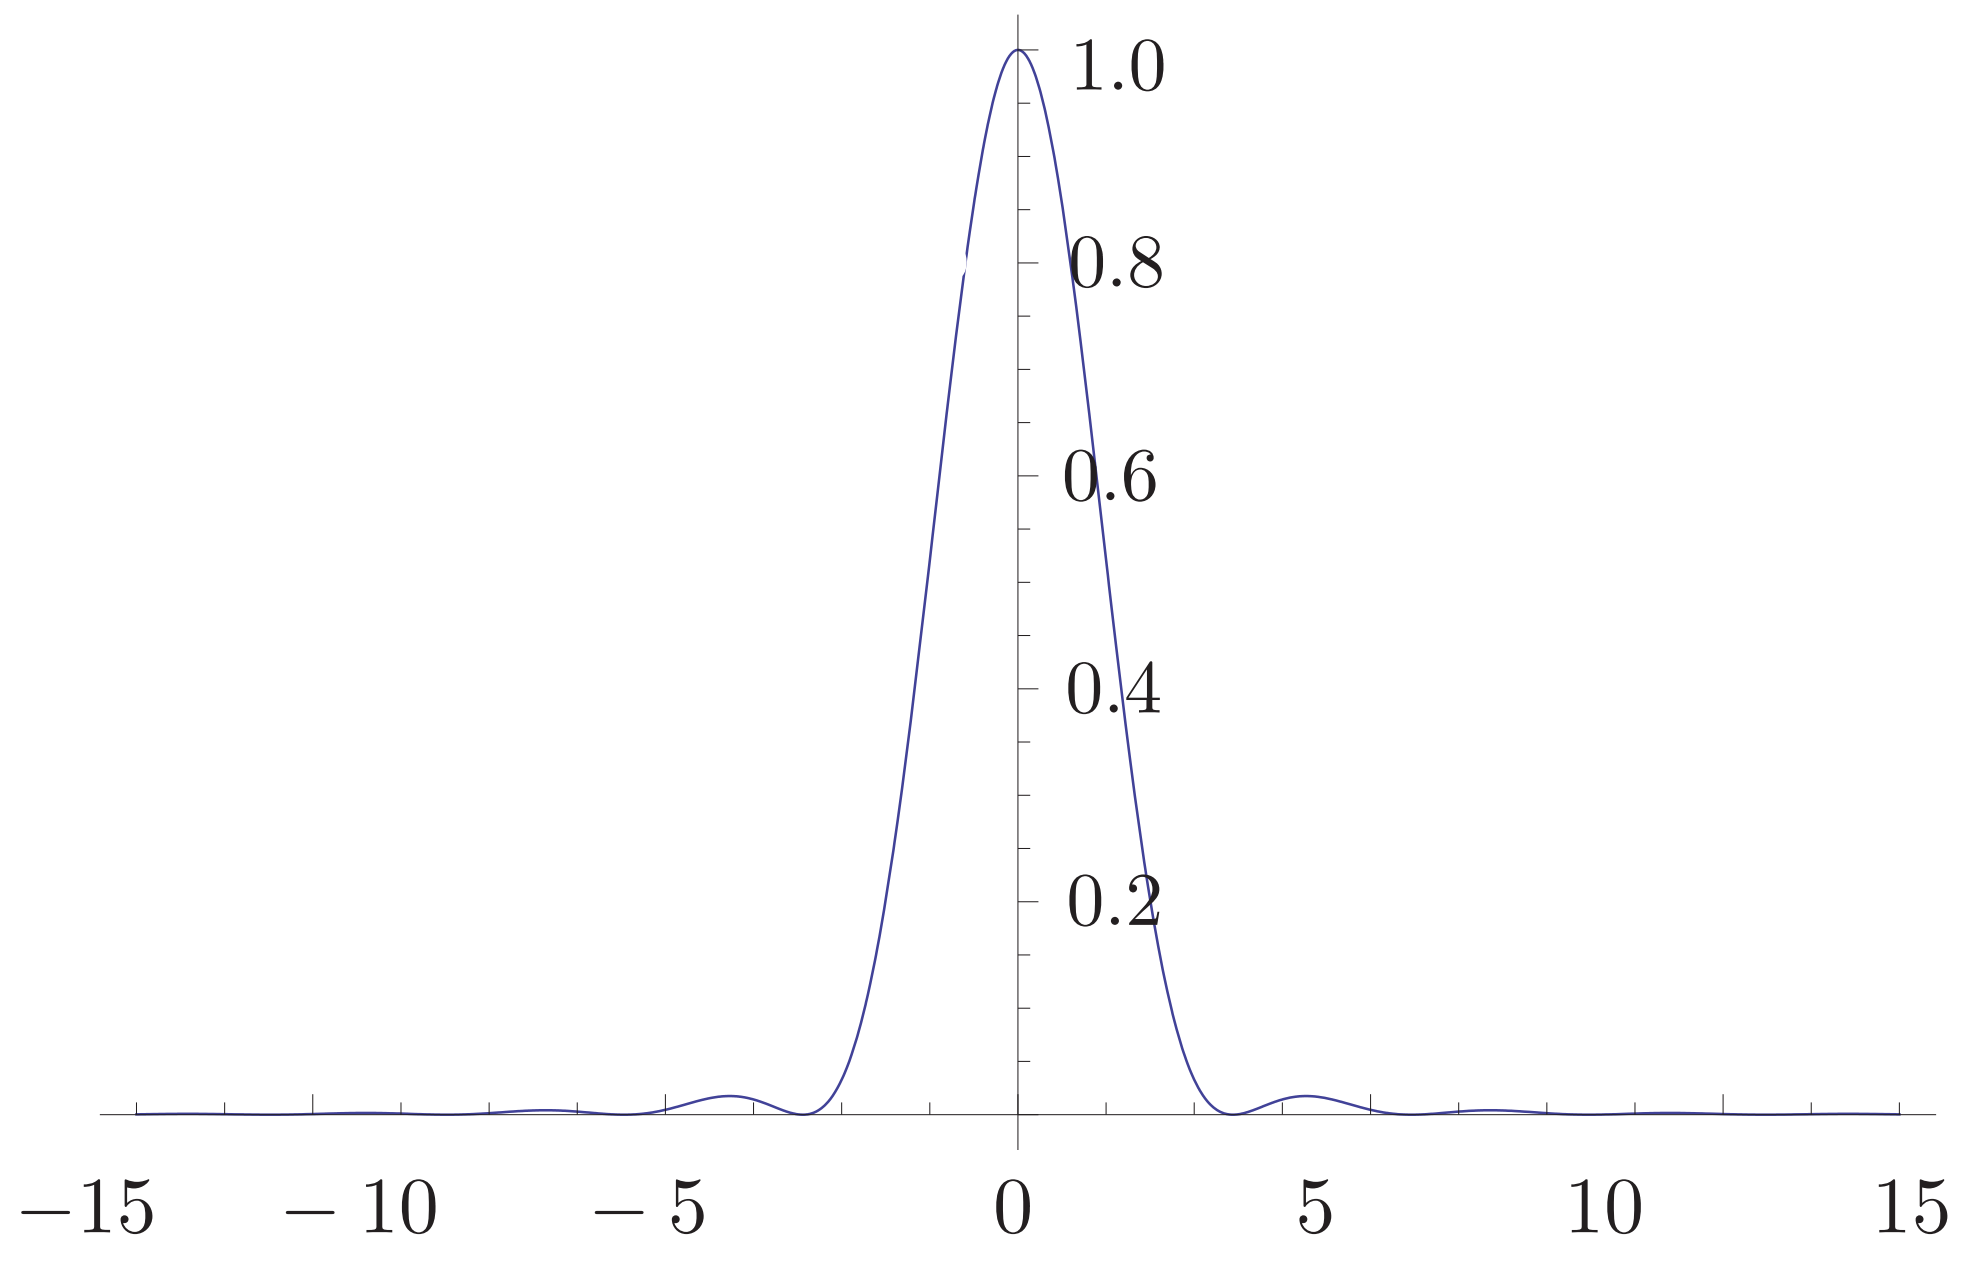
\includegraphics[width=\linewidth]{figures/appendix/circotf.png}
        \caption{Modulation transfer function \(y= \left[ \frac{2J_1(x)}{x} \right]^2\) for a circular aperture \cite{Ivanov2016ElementsOD}.}\label{subfig:mtfcirc}
    \end{subfigure}
    \vskip\baselineskip
    \begin{subfigure}[b]{\subfigwidth}
        \centering
        
\includegraphics[width=\linewidth]{figures/appendix/circpattern.png}
        \caption{Simulated Fraunhofer diffraction from a circular aperture \cite{Ivanov2016ElementsOD}.}\label{subfig:fraunhofcircpattern}
    \end{subfigure}
    \caption{Fraunhofer diffraction through a circular aperture.}\label{fig:fraunhofcirc}
\end{figure}

We now investigate Fraunhofer diffraction through a circular aperture.
%
Using polar coordinates \((\rho, \theta)\) to parameterize the aperture coordinates \((\xi, \eta)\) and \((R, \psi)\) to parameterize the diffraction pattern point \(P\) coordinates \((p, q)\)
%
\begin{align}
    \rho \cos (\theta) = \xi &\quad \rho \sin(\theta) = \eta \\
    R \cos (\psi) = p &\quad R \sin(\psi) = q
\end{align}
%
Note that \(R\), called the \newterm{angular resolution}, represents maximum resolvable distance in the diffraction pattern.
%
We express the argument of the exponential in the integrand of eqn.~\eqref{eqn:fraunhoderapprox}
%
\begin{multline}
    -\iu k (p \xi + q \eta) = -\iu k \rho (p \cos(\theta) + q \sin(\theta))  \\
    = -\iu k \sqrt{p^2 + q^2}\left( \frac{p \cos(\theta)}{\sqrt{p^2+q^2}} + \frac{q \sin(\theta)}{\sqrt{p^2+q^2}}   \right)  \\ 
    = -\iu k \rho R \left(\cos(\psi) \cos(\theta) + \sin(\psi)\sin(\theta) \right) \\
    = -\iu k \rho R \cos(\theta -\psi)
\end{multline}
%
The integral in eqn.~\eqref{eqn:fraunhoderapprox} then becomes 
%
\begin{equation}
    U(R, \psi) \coloneqq C \int\limits_{0}^a \int\limits_{0}^{2\pi} e^{-\iu k \rho R \cos(\theta - \psi)} \rho \dif \rho \dif \theta
\end{equation}
%
where \(a\) is the radius of the aperture.
%
Using \newterm{Bessel functions of the first kind} \(J_0, J_1\) we have 
%
\begin{align}
    U(R) &\coloneqq 2 \pi C \int\limits_0^a J_0(k \rho R) \rho \dif \rho \\ 
    & = \pi C a^2 \frac{2 J_1 (k a R)}{k a R}
\end{align}
%
with intensity (see figure~\ref{subfig:mtfcirc})
%
\begin{equation}
    I(R) \propto \abs{U(R)}^2 = I_0 \left[ \frac{2 J_1 (k a R)}{k a R} \right]^2\label{eqn:circintens}
\end{equation}
%
where \(I_0\) is peak intensity (which happens to be the intensity at the central peak).

Note that the central maximum of eqn.~\eqref{eqn:circintens} comprises 98\% of the transmitted power. 
%
Therefore the effect of a circular aperture is to disperse a point source into a large circular shape (see figure~\ref{subfig:fraunhofcircpattern}).
%
Note also that the first zero appears at \(k a R \approx 1.22\pi\) and so we recover Rayleigh's criterion as 
%
\begin{equation}
    R_{min} \approx 1.22 \frac{\pi}{k a} = 1.22 \frac{\lambda\pi}{2\pi a} = 1.22 \frac{\lambda}{D} 
\end{equation}
%
where \(D = 2a\) the diameter of the aperture.
% \subsection{Automatic Differentiation}\label{subsubsec:autodiff}

% Let
% %
% \begin{align*}
%     F\colon\; \bx \in \mathbb{R}^n \mapsto y \in \mathbb{R}
% \end{align*}
% %
% and decompose \(F\) as
% \begin{equation*}
%     F = D \circ C \circ B \circ A
% \end{equation*}
% %
% where
% %
% \begin{align*}
%     A & \colon\; \bx \in \mathbb{R}^n \mapsto  \bm{a} \in \mathbb{R}^m    \\
%     B & \colon\; \bm{a} \in \mathbb{R}^m \mapsto  \bm{b} \in \mathbb{R}^k \\
%     C & \colon\; \bm{b} \in \mathbb{R}^k \mapsto  \bm{c} \in \mathbb{R}^j \\
%     D & \colon\; \bm{c} \in \mathbb{R}^j \mapsto  y \in \mathbb{R}
% \end{align*}
% %
% Let \(y_0 = F(\bm{x}_0)\) where \(\bx_0 \coloneqq \left( x_{01}, \dots, x_{0n}\right)\).
% %
% Then the gradient of \(F\) evaluated at \(\bx_0\) is
% \begin{equation*}
%     F'(\bm{x}_0) = \evalat[\bigg]{\pdv{y}{\bm{x}}}{\bx = \bx_0}
%     = \left(
%     \evalat[\bigg]{\pdv{y}{x_1}}{x_1 = x_{01}},
%     \;\dots\dots\;,
%     \evalat[\bigg]{\pdv{y}{x_n}}{x_n = x_{0n}}
%     \right)
% \end{equation*}
% %
% Note we are implicitly defining the parameter of \(F' = \pdv{y}{\bx}\) to be \(\bx\).
% %
% This is fine because parameters can be renamed at will\anote{boundvariable} but it's important to keep in mind that \(F'\) is wholly different from \(F\) and could have any other parameter.
% %
% By the chain rule
% \begin{equation*}
%     F'(\bm{x}_0) =  D'(C'(B'(A'(\bx_0))))
% \end{equation*}
% %
% or if we define intermediate values
% %
% \begin{align*}
%     \bm{a}_0 & = A(\bx_0)    \\
%     \bm{b}_0 & = B(\bm{a}_0) \\
%     \bm{c}_0 & = C(\bm{b}_0) \\
%     y_0      & = D(\bm{c}_0)
% \end{align*}
% %
% then
% %
% \begin{equation}
%     F'(\bm{x}_0) =  \evalat[\bigg]{\pdv{y}{\bm{c}}}{\bm{c}=\bm{c}_0} \times\;
%     \evalat[\bigg]{\pdv{\bm{c}}{\bm{b}}}{\bm{b}=\bm{b}_0} \times\;
%     \evalat[\bigg]{\pdv{\bm{b}}{\bm{a}}}{\bm{a}=\bm{a}_0} \times\;
%     \evalat[\bigg]{\pdv{\bm{a}}{\bm{x}}}{\bx=\bx_0} \label{eqn:chainruleproduct}
% \end{equation}
% %
% where now a term like \(\evalat[\big]{\pdv{\bm{b}}{\bm{a}}}{\bm{a}=\bm{a}_0}\) is the \newterm{Jacobian} of \(B\) evaluated at \(\bm{a}_0\):
% %
% \begin{align*}
%     \evalat[\bigg]{\pdv{\bm{b}}{\bm{a}}}{\bm{a}=\bm{a}_0}
%      & = \evalat*{
%         \begin{bmatrix}
%             \pdv{b_1}{a_1} & \cdots & \pdv{b_1}{a_m} \\
%             \vdots         & \ddots & \vdots         \\
%             \pdv{b_k}{a_1} & \cdots & \pdv{b_k}{a_m}
%         \end{bmatrix}
%     }{\bm{a}=\bm{a}_0} \\
%      & \coloneqq
%     \begin{bmatrix}
%         \evalat[\Big]{\pdv{b_1}{a_1}}{a_1 = a_{01}} & \cdots & \evalat[\Big]{\pdv{b_1}{a_m}}{a_m = a_{0m}} \\
%         \\
%         \vdots                                      & \ddots & \vdots                                      \\
%         \\
%         \evalat[\Big]{\pdv{b_k}{a_1}}{a_1 = a_{01}} & \cdots & \evalat[\Big]{\pdv{b_k}{a_m}}{a_m = a_{0m}} \\
%     \end{bmatrix}
% \end{align*}
% %

% The right hand side (RHS) of eqn.~\eqref{eqn:chainruleproduct} is associative; if we want to compute \(F'\) in general we can accumulate products starting from the right or starting from the left:
% %
% \begin{align}
%     F' & = \pdv{y}{\bm{c}}
%     \left( \pdv{\bm{c}}{\bm{b}}
%     \left( \pdv{\bm{b}}{\bm{a}}
%     \pdv{\bm{a}}{\bm{x}}\right)\right) \label{eqn:forwardaccum} \\
%     F' & =  \left( \left( \pdv{y}{\bm{c}}
%     \pdv{\bm{c}}{\bm{b}} \right)
%     \pdv{\bm{b}}{\bm{a}} \right)
%     \pdv{\bm{a}}{\bm{x}} \label{eqn:reverseaccum}
% \end{align}
% %
% Computing \(F'\) as in eqn.~\eqref{eqn:forwardaccum} is called \newterm{forward accumulation} (because it parallels the evaluation order of \(F\)) and, conversely, deriving \(F'\) as in eqn.~\eqref{eqn:reverseaccum} is called \newterm{reverse accumulation}.
% %
% Notice that since \(F\colon\; \mathbb{R}^n  \rightarrow \mathbb{R}\) it's the case that while \(\pdv{\bm{b}}{\bm{a}}\cdot \pdv{\bm{a}}{\bm{x}}\) is a jacobian--jacobian product
% \begin{equation}
%     \pdv{\bm{b}}{\bm{a}}\cdot
%     \pdv{\bm{a}}{\bm{x}} =         \begin{bmatrix}
%         \pdv{b_1}{a_1} & \cdots & \pdv{b_1}{a_m} \\
%         \vdots         & \ddots & \vdots         \\
%         \pdv{b_k}{a_1} & \cdots & \pdv{b_k}{a_m}
%     \end{bmatrix}
%     \cdot
%     \begin{bmatrix}
%         \pdv{a_1}{x_1} & \cdots & \pdv{a_1}{x_n} \\
%         \vdots         & \ddots & \vdots         \\
%         \pdv{a_m}{x_1} & \cdots & \pdv{a_m}{x_n}
%     \end{bmatrix}
% \end{equation}
% %
% while \(\pdv{y}{\bm{c}}\cdot \pdv{\bm{c}}{\bm{b}}\) is a vector--Jacobian product (called a VJP)
% %
% \begin{equation}
%     \pdv{y}{\bm{c}}\cdot
%     \pdv{\bm{c}}{\bm{b}} = \left( \pdv{y}{c_1}, \dots,  \pdv{y}{c_j} \right)
%     \cdot
%     \begin{bmatrix}
%         \pdv{c_1}{b_1} & \cdots & \pdv{c_1}{b_k} \\
%         \vdots         & \ddots & \vdots         \\
%         \pdv{c_j}{b_1} & \cdots & \pdv{c_j}{b_k}
%     \end{bmatrix}
% \end{equation}
% %
% All intermediate products will also be VJPs (for reverse accumulation); in general reverse accumulation is more efficient when the dimension of the domain is greater than the dimension of the range.

% \subsection{Splines}\label{subsubsec:splines}

% A \newterm{spline} is a piecewise defined polynomial function. For example a simple \newterm{order} \(d+1\) spline \(s\) could be defined
% %
% \[
%     s(x) \coloneqq \sum_{i=0}^d \mathbbm{1}_{[k_j, k_{j+1})}P_{ij} \cdot (x - k_j)^i
% \]
% %
% where the \(n+1\) increasing \newterm{knots} \(k_0 < \cdots < k_n\) bracket \(n\) intervals over which the component polynomials are defined, and the \((d+1)\) polynomial coefficients \(P_{ij}\) define the spline (see figure~\ref{fig:cubicspline}) for \(x \in [k_j, k_{j+1})\) (\(\mathbbm{1}\) enforces this\anote{indicator}).
% %
% Splines need not be differentiable (nor even continuous) at the knots but can be specified with such continuity constraints (at the knots).

% The number of degrees of freedom (the dimension of the vector space\anote{vectorspace} of such splines) of a spline over \(n+1\) knots and of order \(d+1\) is the number of polynomial coefficients minus the number of continuity conditions.
% %
% For example if the spline is constrained to be maximally continuous (\(d-1\) times\anote{splinecontconstr}) then the spline has \(d+1\) polynomial coefficients for every one of the \(n\) knot intervals and \(d\) continuity constraints at every one of the \(n-1\) interior knots (continuity constraints cannot be specified at the boundary knots), which implies
% \[
%     n(d+1) - (n-1)d = n+d
% \]
% degrees of freedom.

% A Basis-spline (B-spline) is a spline defined as a linear combination of a particular set of basis functions: the B-spline basis element \(B_{i, d+1}\) of order \(d+1\) (degree \(d\)) over knots \(k_i < \cdots < k_{i+d+1}\) is defined recursively according to the Cox-de Boor recursion formula \cite{de1971subroutine}:
% \begin{align}
%     B_{j,1} (x)   & \coloneqq \mathbbm{1}_{[k_j, k_{j+1})}                         \\
%     B_{j,d+1} (x) & \coloneqq \frac{x-k_j}{k_{j+d} - k_j} B_{j,d} (x)              \\
%                   & \quad+ \frac{k_{j+d+1} - x}{k_{j+d+1} - k_{i+1}} B_{j+1,d} (x)
% \end{align}
% %
% Note that the coefficients
% %
% \[
%     \frac{x-k_j}{k_{j+d} - k_j}
% \]
% %
% and
% %
% \[
%     \frac{k_{j+d+1} - x}{k_{j+d+1} - k_{i+1}}
% \]
% %
% interpolate smoothly between the lower order B-splines \(B_{j,d}, B_{j+1,d}\) as \(x\) goes from \(k_j\) to \(k_{j+d+1}\).

% \begin{figure}
%     \centering
%     \begin{adjustbox}{width=\linewidth}
%         \begin{tikzpicture}
%             \tikzset{
%                 ctrlpoint/.style={%
%                         draw=black,
%                         fill,
%                         circle,
%                         inner sep=0,
%                         minimum width=3pt,
%                     }
%             }
%             \newcommand\Bezier[4]{% \bezier (lowercase 'b') was already defined elsewhere
%                 \node (p1) [ctrlpoint,label=90:\(P_{00}\)] at (#1) {};
%                 \node (p2) [ctrlpoint,label=90:\(P_{01}\)] at (#2) {};
%                 \node (p3) [ctrlpoint,label=90:\(P_{10}\)] at (#3) {};
%                 \node (p4) [ctrlpoint,label=90:\(P_{11}\)] at (#4) {};
%                 \draw [black, dotted] (p1) -- (p2) -- (p3) -- (p4);
%                 \draw [black] (#1) .. controls (#2) and (#3) .. (#4);
%             }
%             \Bezier{0,0}{1,1}{2,-1}{3,0}
%         \end{tikzpicture}
%     \end{adjustbox}
%     \caption{Cubic spline.}
%     \label{fig:cubicspline}
% \end{figure}

% \subsection{Delaunay Triangulation}\label{subsec:delaunay}

% Delaunay triangulation for a set points in the plane is a such that no point in is inside the circumcircle of any triangle in triangulation (see figure~\ref{fig:delaunaycircum}).
% %
% \begin{figure}[htbp]
%     \centering
%     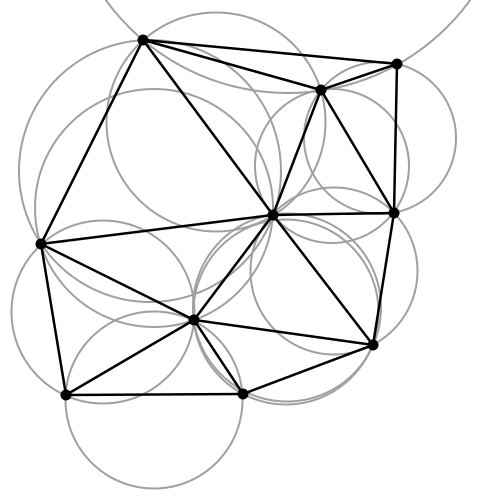
\includegraphics[width=\linewidth]{figures/appendix/delaunay.png}
%     \caption{Delaunay Triangulation.}\label{fig:delaunaycircum}
% \end{figure}
% %
% A local characterization two triangles ABD and BCD with the common edge BD (see figure~\ref{subfig:delauneymismatch}), if the sum of the angles \(\alpha\) and \(\gamma\) is less than or equal to \(\ang{180}\), the triangles meet the Delaunay condition.
% %
% \begin{figure}[htbp]
%     \centering
%     \newcommand*{\subfigwidth}{.8\linewidth}
%     \begin{subfigure}[b]{\subfigwidth}
%         \centering
%         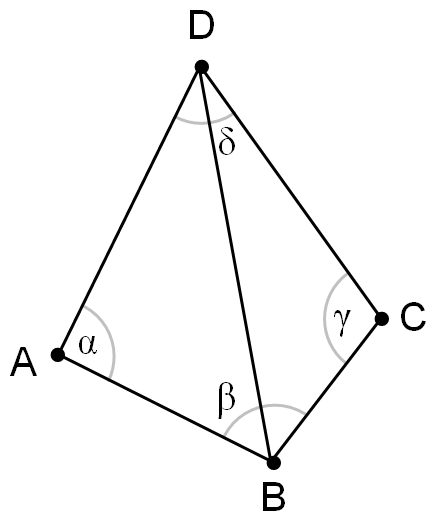
\includegraphics[width=\subfigwidth]{figures/appendix/Delaunay_geometry.png}
%         \caption{This triangulation does not meet the Delaunay condition (the sum of \(\alpha\) and \(\gamma\) is bigger than \(\ang{180}\)).}\label{subfig:delauneymismatch}
%     \end{subfigure}

%     \begin{subfigure}[b]{\subfigwidth}
%         \centering
%         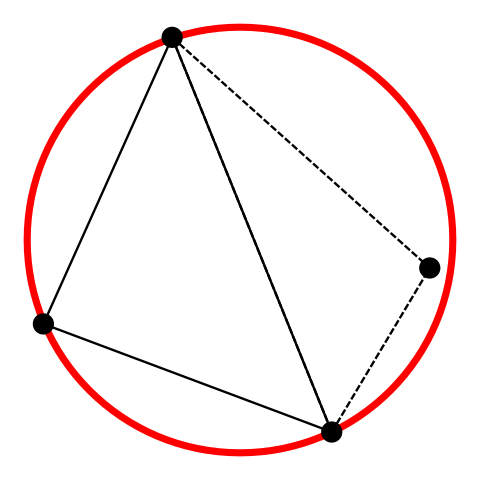
\includegraphics[width=\subfigwidth]{figures/appendix/Point_inside_circle_-_Delaunay_condition_broken.png}
%         \caption{This pair of triangles does not meet the Delaunay condition (the circumcircle contains more than three points).}\label{subfig:delauneyflip}
%     \end{subfigure}

%     \begin{subfigure}[b]{\subfigwidth}
%         \centering
%         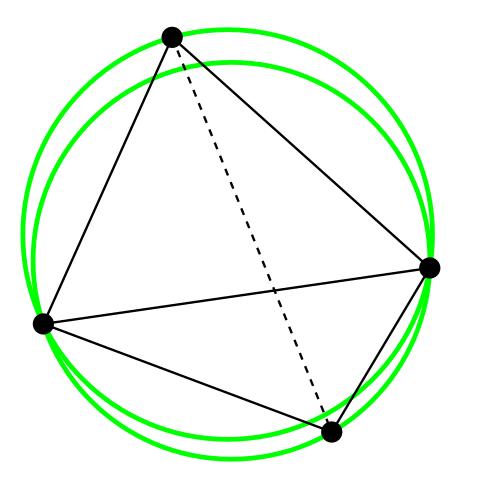
\includegraphics[width=\subfigwidth]{figures/appendix/Edge_Flip_-_Delaunay_condition_ok.png}
%         \caption{Flipping the common edge produces a valid Delaunay triangulation for the four points.}\label{subfig:delauneyfix}
%     \end{subfigure}
%     \caption{Visual Delaunay definition and Flipping.}\label{fig:delauneyflip}
% \end{figure}
% %
% This is an important property because it allows the use of a flipping technique. If two triangles do not meet the Delaunay condition, switching the common edge BD for the common edge AC produces two triangles that do meet the Delaunay condition (see figures~\ref{subfig:delauneyflip}, \ref{subfig:delauneyfix}).
% %
% This leads to a straightforward algorithm: construct any triangulation of the points, and then flip edges until no triangle is non-Delaunay.